%%%%%%%%%%%%%%%%%%%%%%%%%%%%%%%%%%%%%%%%%
%  My documentation report
%  Objetive: Explain what I did and how, so someone can continue with the investigation
%
% Important note:
% Chapter heading images should have a 2:1 width:height ratio,
% e.g. 920px width and 460px height.
%
%%%%%%%%%%%%%%%%%%%%%%%%%%%%%%%%%%%%%%%%%

%----------------------------------------------------------------------------------------
%	PACKAGES AND OTHER DOCUMENT CONFIGURATIONS
%----------------------------------------------------------------------------------------

\documentclass[11pt,fleqn]{book} % Default font size and left-justified equations

\usepackage[top=3cm,bottom=3cm,left=3.2cm,right=3.2cm,headsep=10pt,letterpaper]{geometry} % Page margins

\usepackage{xcolor,lipsum} % Required for specifying colors by name
\definecolor{ocre}{RGB}{51,102,0} 
\definecolor{lightgray}{RGB}{229,229,229} 
% Font Settings
\usepackage{avant} % Use the Avantgarde font for headings
%\usepackage{times} % Use the Times font for headings
\usepackage{mathptmx} % Use the Adobe Times Roman as the default text font together with math symbols from the Sym­bol, Chancery and Com­puter Modern fonts

\usepackage{microtype} % Slightly tweak font spacing for aesthetics
\usepackage[utf8]{inputenc} % Required for including letters with accents
\usepackage[T1]{fontenc} % Use 8-bit encoding that has 256 glyphs


% MATHS PACKAGE
\usepackage{amsmath,tikz}
\usetikzlibrary{matrix}
\newcommand*{\horzbar}{\rule[0.05ex]{2.5ex}{0.5pt}}
\usepackage{calc}

% VERBATIM PACKAGE
\usepackage{verbatim}

% Bibliography
\usepackage[style=alphabetic,sorting=nyt,sortcites=true,autopunct=true,babel=hyphen,hyperref=true,abbreviate=false,backref=true,backend=biber]{biblatex}
\addbibresource{bibliography.bib} % BibTeX bibliography file
\defbibheading{bibempty}{}

%----------------------------------------------------------------------------------------
%	VARIOUS REQUIRED PACKAGES
%----------------------------------------------------------------------------------------

\usepackage{titlesec} % Allows customization of titles

\usepackage{graphicx} % Required for including pictures
\graphicspath{{Pictures/}} % Specifies the directory where pictures are stored

\usepackage{lipsum} % Inserts dummy text

\usepackage{tikz} % Required for drawing custom shapes

\usepackage[english]{babel} % English language/hyphenation

\usepackage{enumitem} % Customize lists
\setlist{nolistsep} % Reduce spacing between bullet points and numbered lists

\usepackage{booktabs} % Required for nicer horizontal rules in tables

\usepackage{eso-pic} % Required for specifying an image background in the title page

%----------------------------------------------------------------------------------------
%	MAIN TABLE OF CONTENTS
%----------------------------------------------------------------------------------------

\usepackage{titletoc} % Required for manipulating the table of contents

\contentsmargin{0cm} % Removes the default margin
% Chapter text styling
\titlecontents{chapter}[1.25cm] % Indentation
{\addvspace{15pt}\large\sffamily\bfseries} % Spacing and font options for chapters
{\color{ocre!60}\contentslabel[\Large\thecontentslabel]{1.25cm}\color{ocre}} % Chapter number
{}  
{\color{ocre!60}\normalsize\sffamily\bfseries\;\titlerule*[.5pc]{.}\;\thecontentspage} % Page number
% Section text styling
\titlecontents{section}[1.25cm] % Indentation
{\addvspace{5pt}\sffamily\bfseries} % Spacing and font options for sections
{\contentslabel[\thecontentslabel]{1.25cm}} % Section number
{}
{\sffamily\hfill\color{black}\thecontentspage} % Page number
[]
% Subsection text styling
\titlecontents{subsection}[1.25cm] % Indentation
{\addvspace{1pt}\sffamily\small} % Spacing and font options for subsections
{\contentslabel[\thecontentslabel]{1.25cm}} % Subsection number
{}
{\sffamily\;\titlerule*[.5pc]{.}\;\thecontentspage} % Page number
[] 

%----------------------------------------------------------------------------------------
%	MINI TABLE OF CONTENTS IN CHAPTER HEADS
%----------------------------------------------------------------------------------------

% Section text styling
\titlecontents{lsection}[0em] % Indendating
{\footnotesize\sffamily} % Font settings
{}
{}
{}

% Subsection text styling
\titlecontents{lsubsection}[.5em] % Indentation
{\normalfont\footnotesize\sffamily} % Font settings
{}
{}
{}
 
%----------------------------------------------------------------------------------------
%	PAGE HEADERS
%----------------------------------------------------------------------------------------

\usepackage{fancyhdr} % Required for header and footer configuration

\pagestyle{fancy}
\renewcommand{\chaptermark}[1]{\markboth{\sffamily\normalsize\bfseries\chaptername\ \thechapter.\ #1}{}} % Chapter text font settings
\renewcommand{\sectionmark}[1]{\markright{\sffamily\normalsize\thesection\hspace{5pt}#1}{}} % Section text font settings
\fancyhf{} \fancyhead[LE,RO]{\sffamily\normalsize\thepage} % Font setting for the page number in the header
\fancyhead[LO]{\rightmark} % Print the nearest section name on the left side of odd pages
\fancyhead[RE]{\leftmark} % Print the current chapter name on the right side of even pages
\renewcommand{\headrulewidth}{0.5pt} % Width of the rule under the header
\addtolength{\headheight}{2.5pt} % Increase the spacing around the header slightly
\renewcommand{\footrulewidth}{0pt} % Removes the rule in the footer
\fancypagestyle{plain}{\fancyhead{}\renewcommand{\headrulewidth}{0pt}} % Style for when a plain pagestyle is specified

% Removes the header from odd empty pages at the end of chapters
\makeatletter
\renewcommand{\cleardoublepage}{
\clearpage\ifodd\c@page\else
\hbox{}
\vspace*{\fill}
\thispagestyle{empty}
\newpage
\fi}

%----------------------------------------------------------------------------------------
%	THEOREM STYLES
%----------------------------------------------------------------------------------------

\usepackage{amsmath,amsfonts,amssymb,amsthm} % For math equations, theorems, symbols, etc

\newcommand{\intoo}[2]{\mathopen{]}#1\,;#2\mathclose{[}}
\newcommand{\ud}{\mathop{\mathrm{{}d}}\mathopen{}}
\newcommand{\intff}[2]{\mathopen{[}#1\,;#2\mathclose{]}}
\newtheorem{notation}{Notation}[chapter]

%%%%%%%%%%%%%%%%%%%%%%%%%%%%%%%%%%%%%%%%%%%%%%%%%%%%%%%%%%%%%%%%%%%%%%%%%%%
%%%%%%%%%%%%%%%%%%%% dedicated to boxed/framed environements %%%%%%%%%%%%%%
%%%%%%%%%%%%%%%%%%%%%%%%%%%%%%%%%%%%%%%%%%%%%%%%%%%%%%%%%%%%%%%%%%%%%%%%%%%
\newtheoremstyle{ocrenumbox}% % Theorem style name
{0pt}% Space above
{0pt}% Space below
{\normalfont}% % Body font
{}% Indent amount
{\small\bf\sffamily\color{ocre}}% % Theorem head font
{\;}% Punctuation after theorem head
{0.25em}% Space after theorem head
{\small\sffamily\color{ocre}\thmname{#1}\nobreakspace\thmnumber{\@ifnotempty{#1}{}\@upn{#2}}% Theorem text (e.g. Theorem 2.1)
\thmnote{\nobreakspace\the\thm@notefont\sffamily\bfseries\color{black}---\nobreakspace#3.}} % Optional theorem note
\renewcommand{\qedsymbol}{$\blacksquare$}% Optional qed square

\newtheoremstyle{blacknumex}% Theorem style name
{5pt}% Space above
{5pt}% Space below
{\normalfont}% Body font
{} % Indent amount
{\small\bf\sffamily}% Theorem head font
{\;}% Punctuation after theorem head
{0.25em}% Space after theorem head
{\small\sffamily{\tiny\ensuremath{\blacksquare}}\nobreakspace\thmname{#1}\nobreakspace\thmnumber{\@ifnotempty{#1}{}\@upn{#2}}% Theorem text (e.g. Theorem 2.1)
\thmnote{\nobreakspace\the\thm@notefont\sffamily\bfseries---\nobreakspace#3.}}% Optional theorem note

\newtheoremstyle{blacknumbox} % Theorem style name
{0pt}% Space above
{0pt}% Space below
{\normalfont}% Body font
{}% Indent amount
{\small\bf\sffamily}% Theorem head font
{\;}% Punctuation after theorem head
{0.25em}% Space after theorem head
{\small\sffamily\thmname{#1}\nobreakspace\thmnumber{\@ifnotempty{#1}{}\@upn{#2}}% Theorem text (e.g. Theorem 2.1)
\thmnote{\nobreakspace\the\thm@notefont\sffamily\bfseries---\nobreakspace#3.}}% Optional theorem note

%%%%%%%%%%%%%%%%%%%%%%%%%%%%%%%%%%%%%%%%%%%%%%%%%%%%%%%%%%%%%%%%%%%%%%%%%%%
%%%%%%%%%%%%% dedicated to non-boxed/non-framed environements %%%%%%%%%%%%%
%%%%%%%%%%%%%%%%%%%%%%%%%%%%%%%%%%%%%%%%%%%%%%%%%%%%%%%%%%%%%%%%%%%%%%%%%%%
\newtheoremstyle{ocrenum}% % Theorem style name
{5pt}% Space above
{5pt}% Space below
{\normalfont}% % Body font
{}% Indent amount
{\small\bf\sffamily\color{ocre}}% % Theorem head font
{\;}% Punctuation after theorem head
{0.25em}% Space after theorem head
{\small\sffamily\color{ocre}\thmname{#1}\nobreakspace\thmnumber{\@ifnotempty{#1}{}\@upn{#2}}% Theorem text (e.g. Theorem 2.1)
\thmnote{\nobreakspace\the\thm@notefont\sffamily\bfseries\color{black}---\nobreakspace#3.}} % Optional theorem note
\renewcommand{\qedsymbol}{$\blacksquare$}% Optional qed square
\makeatother

% Defines the theorem text style for each type of theorem to one of the three styles above
\newcounter{dummy} 
\numberwithin{dummy}{section}
\theoremstyle{ocrenumbox}
\newtheorem{theoremeT}[dummy]{Theorem}
\newtheorem{problem}{Problem}[chapter]
\newtheorem{exerciseT}{Exercise}[chapter]
\theoremstyle{blacknumex}
\newtheorem{exampleT}{Example}[chapter]
\theoremstyle{blacknumbox}
\newtheorem{vocabulary}{Vocabulary}[chapter]
\newtheorem{definitionT}{Definition}[section]
\newtheorem{corollaryT}[dummy]{Corollary}
\theoremstyle{ocrenum}
\newtheorem{proposition}[dummy]{Proposition}

%----------------------------------------------------------------------------------------
%	DEFINITION OF COLORED BOXES
%----------------------------------------------------------------------------------------

\RequirePackage[framemethod=default]{mdframed} % Required for creating the theorem, definition, exercise and corollary boxes

% Theorem box
\newmdenv[skipabove=7pt,
skipbelow=7pt,
backgroundcolor=black!5,
linecolor=ocre,
innerleftmargin=5pt,
innerrightmargin=5pt,
innertopmargin=5pt,
leftmargin=0cm,
rightmargin=0cm,
innerbottommargin=5pt]{tBox}

% Exercise box	  
\newmdenv[skipabove=7pt,
skipbelow=7pt,
rightline=false,
leftline=true,
topline=false,
bottomline=false,
backgroundcolor=ocre!10,
linecolor=ocre,
innerleftmargin=5pt,
innerrightmargin=5pt,
innertopmargin=5pt,
innerbottommargin=5pt,
leftmargin=0cm,
rightmargin=0cm,
linewidth=4pt]{eBox}	

% Definition box
\newmdenv[skipabove=7pt,
skipbelow=7pt,
rightline=false,
leftline=true,
topline=false,
bottomline=false,
linecolor=ocre,
innerleftmargin=5pt,
innerrightmargin=5pt,
innertopmargin=0pt,
leftmargin=0cm,
rightmargin=0cm,
linewidth=4pt,
innerbottommargin=0pt]{dBox}	

% Corollary box
\newmdenv[skipabove=7pt,
skipbelow=7pt,
rightline=false,
leftline=true,
topline=false,
bottomline=false,
linecolor=gray,
backgroundcolor=black!5,
innerleftmargin=5pt,
innerrightmargin=5pt,
innertopmargin=5pt,
leftmargin=0cm,
rightmargin=0cm,
linewidth=4pt,
innerbottommargin=5pt]{cBox}

% Creates an environment for each type of theorem and assigns it a theorem text style from the "Theorem Styles" section above and a colored box from above
\newenvironment{theorem}{\begin{tBox}\begin{theoremeT}}{\end{theoremeT}\end{tBox}}
\newenvironment{exercise}{\begin{eBox}\begin{exerciseT}}{\hfill{\color{ocre}\tiny\ensuremath{\blacksquare}}\end{exerciseT}\end{eBox}}				  
\newenvironment{definition}{\begin{dBox}\begin{definitionT}}{\end{definitionT}\end{dBox}}	
\newenvironment{example}{\begin{exampleT}}{\hfill{\tiny\ensuremath{\blacksquare}}\end{exampleT}}		
\newenvironment{corollary}{\begin{cBox}\begin{corollaryT}}{\end{corollaryT}\end{cBox}}	

%----------------------------------------------------------------------------------------
%	REMARK ENVIRONMENT
%----------------------------------------------------------------------------------------

\newenvironment{remark}{\par\vspace{10pt}\small % Vertical white space above the remark and smaller font size
\begin{list}{}{
\leftmargin=35pt % Indentation on the left
\rightmargin=25pt}\item\ignorespaces % Indentation on the right
\makebox[-2.5pt]{\begin{tikzpicture}[overlay]
\node[draw=ocre!60,line width=1pt,circle,fill=ocre!25,font=\sffamily\bfseries,inner sep=2pt,outer sep=0pt] at (-15pt,0pt){\textcolor{ocre}{R}};\end{tikzpicture}} % Orange R in a circle
\advance\baselineskip -1pt}{\end{list}\vskip5pt} % Tighter line spacing and white space after remark

%----------------------------------------------------------------------------------------
%	SECTION NUMBERING IN THE MARGIN
%----------------------------------------------------------------------------------------

\makeatletter
\renewcommand{\@seccntformat}[1]{\llap{\textcolor{ocre}{\csname the#1\endcsname}\hspace{1em}}}                    
\renewcommand{\section}{\@startsection{section}{1}{\z@}
{-4ex \@plus -1ex \@minus -.4ex}
{1ex \@plus.2ex }
{\normalfont\large\sffamily\bfseries}}
\renewcommand{\subsection}{\@startsection {subsection}{2}{\z@}
{-3ex \@plus -0.1ex \@minus -.4ex}
{0.5ex \@plus.2ex }
{\normalfont\sffamily\bfseries}}
\renewcommand{\subsubsection}{\@startsection {subsubsection}{3}{\z@}
{-2ex \@plus -0.1ex \@minus -.2ex}
{.2ex \@plus.2ex }
{\normalfont\small\sffamily\bfseries}}                        
\renewcommand\paragraph{\@startsection{paragraph}{4}{\z@}
{-2ex \@plus-.2ex \@minus .2ex}
{.1ex}
{\normalfont\small\sffamily\bfseries}}

%----------------------------------------------------------------------------------------
%	HYPERLINKS IN THE DOCUMENTS
%----------------------------------------------------------------------------------------

% For an unclear reason, the package should be loaded now and not later
\usepackage{hyperref}
\hypersetup{hidelinks,backref=true,pagebackref=true,hyperindex=true,colorlinks=false,breaklinks=true,urlcolor= ocre,bookmarks=true,bookmarksopen=false,pdftitle={Title},pdfauthor={Author}}

%----------------------------------------------------------------------------------------
%	CHAPTER HEADINGS
%----------------------------------------------------------------------------------------

% The set-up below should be (sadly) manually adapted to the overall margin page septup controlled by the geometry package loaded in the main.tex document. It is possible to implement below the dimensions used in the goemetry package (top,bottom,left,right)... TO BE DONE

\newcommand{\thechapterimage}{}
\newcommand{\chapterimage}[1]{\renewcommand{\thechapterimage}{#1}}

% Numbered chapters with mini tableofcontents
\def\thechapter{\arabic{chapter}}
\def\@makechapterhead#1{
\thispagestyle{empty}
{\centering \normalfont\sffamily
\ifnum \c@secnumdepth >\m@ne
\if@mainmatter
\startcontents
\begin{tikzpicture}[remember picture,overlay]
\node at (current page.north west)
{\begin{tikzpicture}[remember picture,overlay]
\node[anchor=north west,inner sep=0pt] at (0,0) {\includegraphics[width=\paperwidth]{\thechapterimage}};
%%%%%%%%%%%%%%%%%%%%%%%%%%%%%%%%%%%%%%%%%%%%%%%%%%%%%%%%%%%%%%%%%%%%%%%%%%%%%%%%%%%%%
% Commenting the 3 lines below removes the small contents box in the chapter heading
%\fill[color=ocre!10!white,opacity=.6] (1cm,0) rectangle (8cm,-7cm);
%\node[anchor=north west] at (1.1cm,.35cm) {\parbox[t][8cm][t]{6.5cm}{\huge\bfseries\flushleft \printcontents{l}{1}{\setcounter{tocdepth}{2}}}};
\draw[anchor=west] (5cm,-9cm) node [rounded corners=20pt,fill=ocre!10!white,text opacity=1,draw=ocre,draw opacity=1,line width=1.5pt,fill opacity=.6,inner sep=12pt]{\huge\sffamily\bfseries\textcolor{black}{\thechapter. #1\strut\makebox[22cm]{}}};
%%%%%%%%%%%%%%%%%%%%%%%%%%%%%%%%%%%%%%%%%%%%%%%%%%%%%%%%%%%%%%%%%%%%%%%%%%%%%%%%%%%%%
\end{tikzpicture}};
\end{tikzpicture}}
\par\vspace*{230\p@}
\fi
\fi}

% Unnumbered chapters without mini tableofcontents (could be added though) 
\def\@makeschapterhead#1{
\thispagestyle{empty}
{\centering \normalfont\sffamily
\ifnum \c@secnumdepth >\m@ne
\if@mainmatter
\begin{tikzpicture}[remember picture,overlay]
\node at (current page.north west)
{\begin{tikzpicture}[remember picture,overlay]
\node[anchor=north west,inner sep=0pt] at (0,0) {\includegraphics[width=\paperwidth]{\thechapterimage}};
\draw[anchor=west] (5cm,-9cm) node [rounded corners=20pt,fill=ocre!10!white,fill opacity=.6,inner sep=12pt,text opacity=1,draw=ocre,draw opacity=1,line width=1.5pt]{\huge\sffamily\bfseries\textcolor{black}{#1\strut\makebox[22cm]{}}};
\end{tikzpicture}};
\end{tikzpicture}}
\par\vspace*{230\p@}
\fi
\fi
}
\makeatother % Insert the commands.tex file which contains the majority of the structure behind the template

\begin{document}

\let\cleardoublepage\clearpage

%----------------------------------------------------------------------------------------
%	TITLE PAGE
%----------------------------------------------------------------------------------------

\begingroup
\thispagestyle{empty}
\AddToShipoutPicture*{\put(0,0){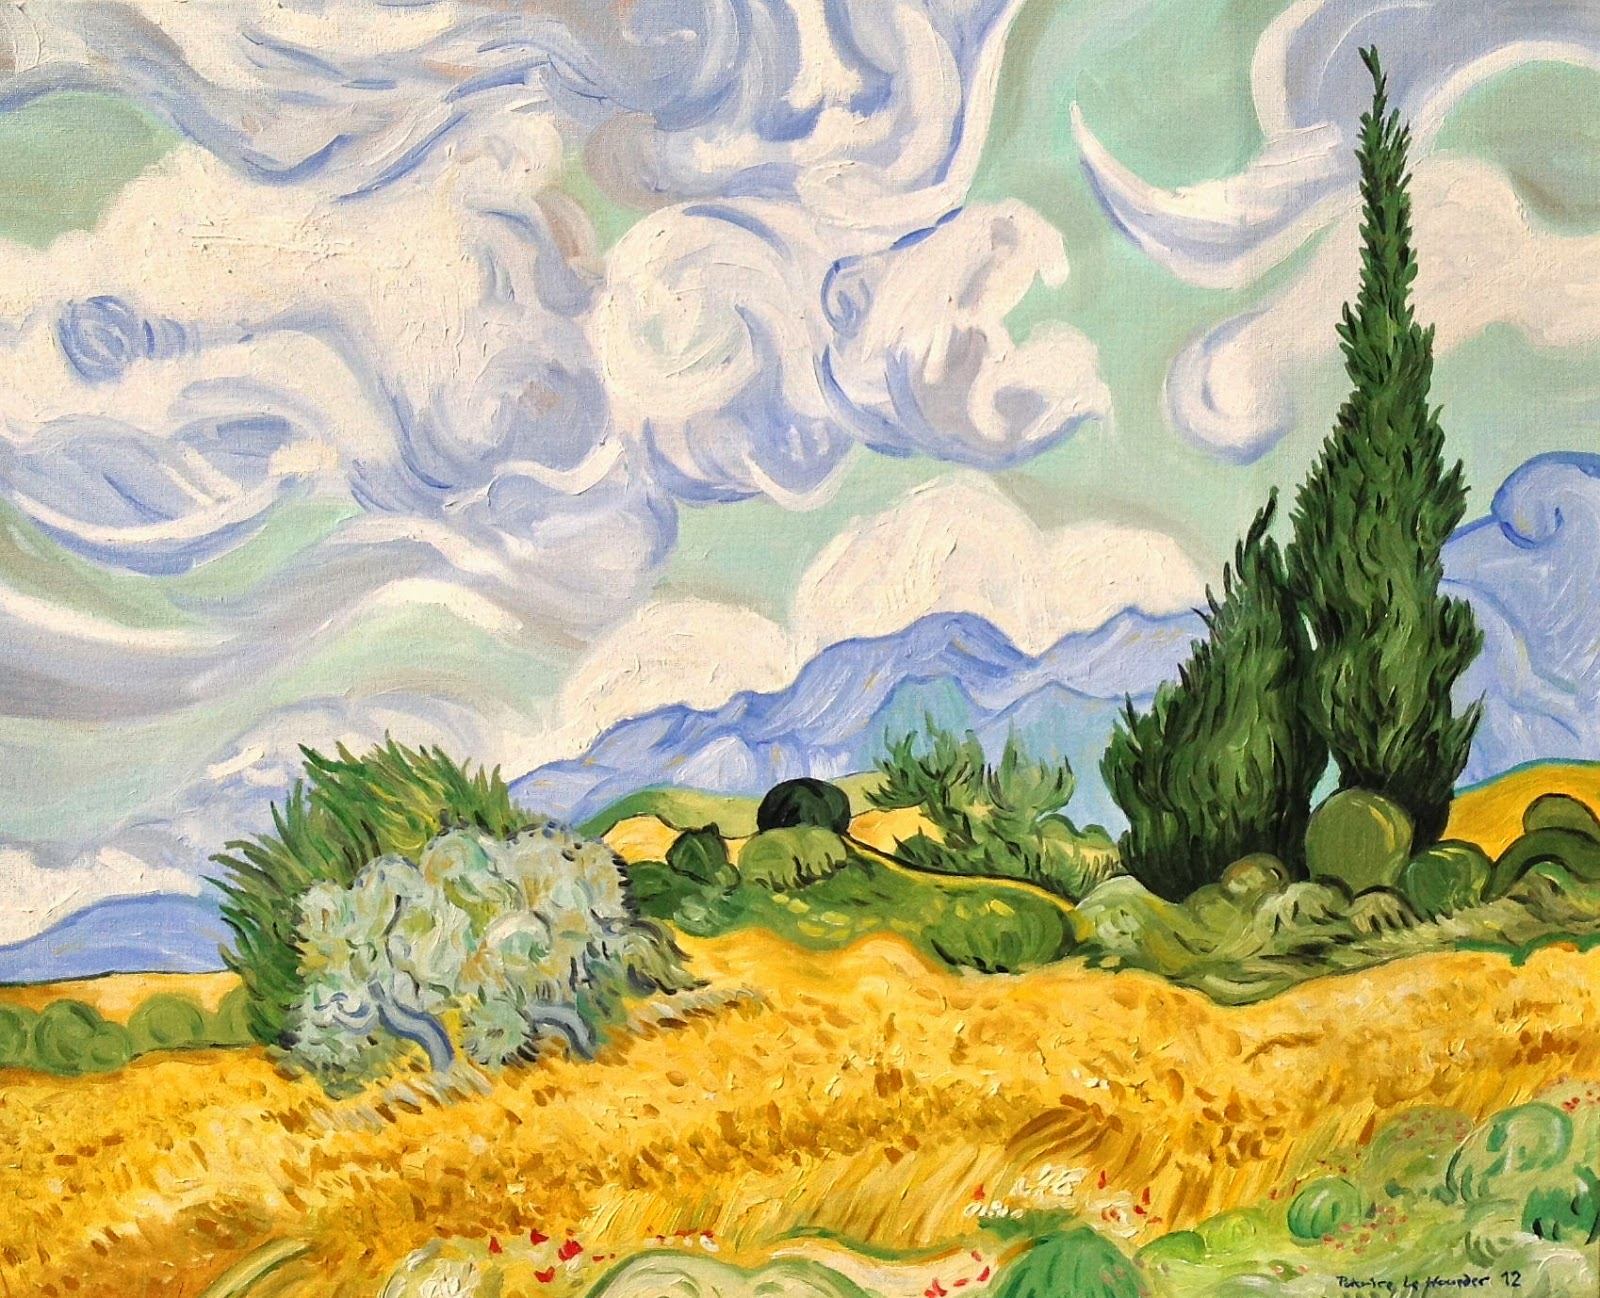
\includegraphics[scale=1.25]{v}}} % Image background
\centering
\vspace*{5cm}
\par\normalfont\fontsize{35}{35}\sffamily\selectfont
\textbf{MODELE LINEAIRE A EFFETS MIXTES\\ THEORIE \& APPLICATION }\\
{\LARGE }\par % Book title
\vspace*{1cm}
{\Huge Amin EL GAREH et Bezeid CHEICK-MOHAMED-LMAMI}\par % Author name
\endgroup

%----------------------------------------------------------------------------------------
%	COPYRIGHT PAGE
%----------------------------------------------------------------------------------------

\newpage
~\vfill
\thispagestyle{empty}

%\noindent Copyright \copyright\ 2014 Andrea Hidalgo\\ % Copyright notice

\noindent \textsc{Projet Janvier-Mars 2015, Université de Bourgogne}\\

\noindent Ce projet a été encadré par Hervé CARDOT.\\ % License information

\noindent \textit{Publié le 30 Mars 2015} % Printing/edition date

%----------------------------------------------------------------------------------------
%	TABLE OF CONTENTS
%----------------------------------------------------------------------------------------

\chapterimage{pano-5.jpg} % heading image

\pagestyle{empty} % No headers

\renewcommand\contentsname{Table des Matières}
\renewcommand{\bibname}{Bibliographie}
\tableofcontents% Print the table of contents itself

%\cleardoublepage % Forces the first chapter to start on an odd page so it's on the right

\pagestyle{fancy} % Print headers again

%----------------------------------------------------------------------------------------
%	CHAPTER 1
%----------------------------------------------------------------------------------------

\chapterimage{pano-5.jpg} % Chapter heading image

\chapter{Introduction}

\section{Motivation}\index{Motivation}

  \vspace{1em}

 Le modèle linéaire mixte a été mis en oeuvre dès les années 1950, essentiellement dans
le domaine de la génétique animale (réf.       Henderson$^{\textbf{[5]}}$). Il n’a toutefois
connu une utilisation plus générale qu’au cours des années 1990, en relation avec le
développement de nouvelles procédures de calcul dans le cadre des logiciels statistiques. L’utilisation du modèle linéaire mixte soulève, par rapport aux modèles classiques d’analyse de la variance, un certain nombre de difficultés particulières, tant en ce qui concerne l’estimation des différents paramètres que la réalisation des tests d’hypothèses. Des informations peuvent être trouvées à ce sujet
dans les articles de Littell [2002], McLean et al. [1991], et Piepho et al. [2003], et dans les
livres de Demidenko [2004], McCulloch et Searle [2001], 

  \vspace{2em}

\section{Modèle linéaire mixte gaussien à K facteurs aléatoires}

  \vspace{1em}
  
  On appelle modèle mixte un modèle statistique dans lequel on considère à la fois des facteurs à effets fixes (qui vont intervenir au niveau de la moyenne du modèle) et des facteurs à effets aléatoires (qui vont intervenir au niveau de la variance du modèle). Un modèle est dit mixte lorsqu’il y a au moins un facteur de chaque nature. Dans le cadre de ce rapport, nous ne considérons
que des modèles linéaires gaussiens mixtes unidimensionnel à K facteurs aléatoires indépendants plus une résiduelle, mais la notion de modèle mixte se rencontre également dans d’autres contextes, notamment dans le modèle linéaire généralisé.

 \vspace{1em}
 
 Un modèle linéaire à effets mixtes est un modèle (réf. Laird et Ware$^{\textbf{[2]}}$) qui satisfait:

\begin{equation}
\fbox{$
Y=X\beta+\sum_{k=1}^{K} Z_k \gamma_k+\epsilon
$}
\end{equation}

\vspace{1em}

avec $(\gamma_k)_{k=1,...,K}$ le kième vecteur aléatoire et $\epsilon$ le vecteur des résidus.

  \vspace{1em} 
  
$\bullet\quad \gamma_k=\left[
  \begin{array}{ c }
     \gamma_{k1}  \\
     \vdots   \\
     \gamma_{k q_k}  \\ 
  \end{array} \right]_{q_k,1}$  \quad où \: $\gamma_{k1},..., \gamma_{k q_k}\hookrightarrow\mathcal{N}(0,\sigma_k^2)$ \: et indépendantes les unes des autres.

\vspace{1em}
  
  Le vecteur aléatoire $\gamma_k$ est gaussien puisque pour tout $c=(c_1, ... ,c_{q_k})'\in \mathbb{R}^{q_k}$ \\ la variable
  $\sum_{i=1}^{q_k} c_i\gamma_{k i}= c'\gamma_k $ est une variable réelle gaussienne. $\gamma_k$ est donc normalement distribué,\\ 
  $\gamma_k\hookrightarrow\mathcal{N}(0,\Sigma_k)$ de matrice de covariance $\Sigma_k=\sigma_k^2 \: I_{q_k}$ 
  
\vspace{1em}

$\bullet \quad \epsilon=\left[
  \begin{array}{ c }
     \epsilon_{1}  \\
     \vdots   \\
     \epsilon_{n}  \\ 
  \end{array} \right]_{n,1}$  \quad où \: $\epsilon_{1},..., \epsilon_{n}\hookrightarrow\mathcal{N}(0,\sigma_{\epsilon}^2)$ \: et indépendantes les unes des autres.

\vspace{1em}


$\bullet \quad X=\left[
  \begin{array}{ c c c c }
     |  & | & & | \\
     1 & x_1 & ... & x_p  \\
     |  & | & & |
  \end{array} \right]_{n,p+1}$ \quad $\beta=\left[
  \begin{array}{ c }
     \alpha  \\
     \beta_1   \\
      \vdots  \\
      \beta_p  
  \end{array} \right]_{p+1,1} $
  
  \vspace{1em}

$X \in \mathcal{M}_{n,p+1}(\mathbb{R})$ est la matrice formée d'une colonne $1_n$ et de variables explicatives fixées $x_j$.\\ 
$\beta$ est le vecteur de $\mathbb{R}^{p+1}$ qui réunit la constante de régression $\alpha$ et les coefficients $\beta_j$  des variables à effets fixes. Tandis que les matrices $Z_k$ dans $\mathcal{M}_{n,q_k}(\mathbb{R})$ et les vecteurs $\gamma_k$ de $\mathbb{R}^{q_k}$ jouent un rôle pour les composantes aléatoires du modèle.

  \vspace{1em}

\begin{proposition}[Distribution du vecteur à expliquer]

Y est normalement distribué de moyenne  $\mu=X\beta$ et de matrice de covariance $V=\sum_{k=1}^{K} Z_k \sigma_k^2 Z_k'+\sigma^2_{\epsilon} I_{n}$  supposée symétrique, définie positive. 


\end{proposition}

\vspace{1em}

\textit{\textbf{Demonstration.}}

\vspace{0.5em}

\textit{Le vecteur $Y=(y_1,...,y_n)'$ est un vecteur gaussien de $\mathbb{R}^{n}$ puisque pour tout $c=(c_1, ... ,c_{n})'\in \mathbb{R}^{n}$ la variable $\sum_{i=1}^{n}c_i y_i=c'Y=c'(X\beta+\sum_{k=1}^{K} Z_k \gamma_k+\epsilon)=c'X\beta+c'\sum_{k=1}^{K} Z_k \gamma_k+c'\epsilon$ est une variable réelle gaussienne, car $c'X\beta$ est un réel et $c'\sum_{k=1}^{K} Z_k \gamma_k+c'\epsilon$ est une somme de variables réelles gaussiennes.}

\vspace{1em}

\textit{$Y$ est de moyenne $\mu$ et de matrice de covariance $V$ tel que:}

\vspace{1em}

\textit{$\mu=\mathbb{E}[Y] = \mathbb{E}[X\beta]+\sum_{k=1}^{K}\mathbb{E}[Z_k \gamma_k]+\mathbb{E}[\epsilon]  = X\beta$ \quad  (car $X$ est déterministe)}

\vspace{1em}

\begin{align*}
V&=Var(Y) \\
&= Var(X\beta)+ \sum_{k=1}^{K} Var(Z_k \gamma_k)+Var(\epsilon) \\
&= \sum_{k=1}^{K} Z_k\:Var(\gamma_k)\:Z_k'+\sigma^2_{\epsilon} I_{n}\\
&=\sum_{k=1}^{K} Z_k \sigma_k^2 Z_k'+\sigma^2_{\epsilon} I_{n} \quad\quad\quad \blacksquare
\end{align*}


\newpage


   
%%%%%%%%%%%%%%%%%%%%%%%%%%%%%%%%%%%%%%%%%%%%%%%
%%%%%%%%%%%%%%%%%%%%%%%%%%%%%%%%%%%%%%%%%%%%%%%
\chapterimage{pano-5.jpg} % Chapter heading image

\chapter{Méthode ML}


%%%%%%%%%%%%%%%%%%%%%%%%%%%%%%%%%%%%%%%%%%%%%%%
\vspace{1em}

L’idée fondamentale de l’estimation par maximum de vraisemblance dite ML ("Maximum Likelihood") est, comme le nom l’implique, de trouver un ensemble d’estimations de paramètres,\\ 
appelé $\hat{\theta}$, telles que la vraisemblance d’avoir obtenu l’échantillon que nous utilisons soit maximisée. Nous signifions par là que la densité de probabilité jointe pour le modèle que l’on estime est évaluée aux valeurs observées de la (des) variable(s) dépendante(s) et traitée comme une fonction de paramètres du modèle. Le vecteur $\hat{\theta}$ des estimations ML donne alors
le maximum de cette fonction. Ce principe d’estimation est très largement applicable: si nous pouvons écrire la densité jointe de l’échantillon, nous pouvons en principe utiliser le maximum de vraisemblance, soumis bien sûr à certaines conditions de régularité. 

\vspace{1em}

\section{Construction des estimateurs}

\vspace{1em}

On rappelle que le cadre général d'étude est: 

\begin{equation*} 
Y=X\beta+\sum_{k=1}^{K} Z_k \gamma_k+\epsilon 
\end{equation*}

avec \: $ Y\hookrightarrow\mathcal{N}(X\beta,V)$ \:de matrice de covariance $V=\sum_{k=1}^{K} \sigma_k^2 Z_k  Z_k'+\sigma_{\epsilon}^2 I_{n}$

  \vspace{1em}
 Si $Z_k$ est de plein rang alors $V$ est inversible, de ce fait $Y$ admet une densité par rapport à la mesure de Lebesgue $\lambda_{n}$, la fonction $f_{Y} : \mathbb{R}^{n} \rightarrow \mathbb{R}_{+}^{*}$ est définie par:

\begin{equation*}
\fbox{$
\forall\:\: Y \in \mathbb{R}^{n}$, $f_{Y}(Y)=\frac{1}{(2\pi)^{\frac{n}{2}}\sqrt{det(V)}}exp\left(-\frac{1}{2}(Y-X\beta)'\:V^{-1}\:(Y-X\beta)\right) 
$}
\end{equation*}

\vspace{1em}

On note $\alpha=(\sigma_1^2,...,\sigma_K^2,\sigma_{\epsilon}^2)$.


\vspace{1em}

La vraisemblance $L$ est considéré ici comme une fonction dépendante du paramètre $\theta=(\beta',\alpha)$.


\begin{equation*}
\textit{L}(Y,\theta) \:=\:  f_{Y}(Y) \:=\:  (2\pi)^{-\frac{n}{2}} det(V)^{-\frac{1}{2}} \exp\left(-\frac{1}{2}(Y-X\beta)'\:V^{-1}\:(Y-X\beta)\right)
\end{equation*}

\vspace{1em}

Le logarithme de la vraisemblance $L$, dite logvraisemblance est donné par:

\begin{align*}
ln(\textit{L}(Y,\theta)) &= ln(\: f_{Y}(Y) \:)\\
                        &= ln\left(\: (2\pi)^{-\frac{n}{2}} det(V)^{-\frac{1}{2}} \exp\left(-\frac{1}{2}(Y-X\beta)'\:V^{-1}\:(Y-X\beta)\right) \: \right) \\
						&= ln(\:(2\pi)^{-\frac{n}{2}}\:) + ln(\:det(V)^{-\frac{1}{2}}\:) -\frac{1}{2} (Y-X\beta)'\:V^{-1}\:(Y-X\beta) 
\end{align*}


\begin{equation}
\fbox{$
 ln(\textit{L}(Y,\theta)) \;=\: -\frac{n}{2} ln(2\pi) -\frac{1}{2} ln(\:det(V)\:) -\frac{1}{2}  (Y-X\beta)'\:V^{-1}\:(Y-X\beta)
 $}
\end{equation}

\vspace{2em}

%%%%%%
\subsection{Estimation du coefficient $\beta$}

\vspace{2em}

On s'intéresse au terme de (2.1) ne faisant intervenir que le coefficient $\beta$, et on développe l'expression ainsi retenue

$$ -\frac{1}{2} \:\left[\:\: Y\textnormal{'}\:V^{-1}\:\: Y \:\:-\:\: Y\textnormal{'} \:V\:\: X\beta \:\:-\:\: (X\beta)'\:V^{-1}\:\: Y \:\:+\:\: (X\beta)' \:V\:\: X\beta \:\:\right]$$ 

\vspace{1em}

En retenant toujours que les termes faisant intervenir $\beta$ et en remarquant que\\ $Y\textnormal{'}\: V^{-1}\:\:X\beta \:=\: (X\beta)\textnormal{'}\:V^{-1}\:\: Y$ on obtient l'expression suivante:

\begin{equation}
-\frac{1}{2}  \:\left[\: -2\: Y\textnormal{'} \:V^{-1}\:\: X\beta + (X\beta)' \:V^{-1}\:\: X\beta \:\right]
\end{equation}

\vspace{1em}

Puisque l'on souhaite calculer $\frac{\delta ln(\:\textit{L}(Y,\theta)\:)}{\delta\beta}$, alors on dérive (2.2) suivant $\beta$

\begin{align*}
\frac{\delta ln(\:\:\textit{L}(Y,\theta)\:)}{\delta\beta} &= \frac{\delta \left[ -\frac{1}{2} \:\left[\: -2\: Y\textnormal{'} \:V^{-1}\:\: X\beta \:\:+\:\: (X\beta)' \:V^{-1}\:\: X\beta \:\right] \:\: \right] }{\delta\beta} \\
&=  \frac{  \delta \left[\:  Y\textnormal{'} \:V^{-1}\:\: X\beta \:\right] }{\delta\beta} \:-\: \frac{1}{2}  \frac{\delta \left[\:  (X\beta)' \:V^{-1} \:\: X\beta \:\right] }{\delta\beta}\\
&= Y\textnormal{'} \:V^{-1}\:\: X \:\:-\:\: X\textnormal{'} \:V^{-1}\:\: X\beta
\end{align*}

\vspace{1em}

Et en remarquant que \quad $Y\textnormal{'} \:V^{-1}\:\: X\:=\:X\textnormal{'} \:V^{-1}\:\: Y$, on a:

\begin{equation}
 \fbox{$
\frac{\delta ln(\:\:\textit{L}(Y,\theta)\:)}{\delta\beta} \:=\: X\textnormal{'} \:V^{-1}\:\: Y \:\:-\:\: X\textnormal{'} \:V^{-1}\:\: X\beta
$}
\end{equation}

\vspace{1em}

\begin{align*}
\frac{\delta ln(\:\textit{L}(Y,\theta)\:)}{\delta\beta}=0 &\Leftrightarrow \: X\textnormal{'} \:V^{-1}\:\: Y \:\:-\:\:  X\textnormal{'} \:V^{-1}\:\: X\beta = 0 \\
& \Leftrightarrow \:   X\textnormal{'} \:V^{-1}\:\: X\beta \:=\:  X\textnormal{'} \:V^{-1}\:\: Y\\
& \Leftrightarrow \: \beta \: = \: \left(  X\textnormal{'}\:V^{-1}\:\: X \right)^{-1}  \: X\textnormal{'} \:V^{-1}\:\: Y
\end{align*}

\vspace{1em}

$\beta=\hat{\beta}$ est un maximum local si la condition suffisante: $\frac{\delta^2 ln(\:\textit{L}(Y,\theta)\:)}{\delta\beta^2}<0$ est vérifiée.


\begin{equation} 
\fbox{$
\hat{\beta}\:=\:\left(  X\textnormal{'}\:V^{-1} \: X \right)^{-1} \quad X\textnormal{'} \:V^{-1}\: Y 
$}
\end{equation}

\begin{equation}
\fbox{$
\frac{\delta^2 ln(\:\textit{L}(Y,\theta)\:)}{\delta\beta^2} \:=\: -\: X\textnormal{'} \:V^{-1}\:\: X
\:= - X\textnormal{'} \: \left( \: \sum_{k=1}^{K} \sigma_k^2 Z_k Z_k'+\sigma_{\epsilon}^2 I_{n} \:\right)^{-1}\: X $}
\end{equation}

\vspace{2em} 


\subsection{Estimation des variances $\alpha_k$}

\vspace{2em}

Cette fois on s'intéresse qu'aux termes de (2.1) faisant intervenir $\alpha_k$ c'est à dire: 

\begin{equation}
-\frac{1}{2} ln(\:det(V)\:) -\frac{1}{2}  (Y-X\beta)'\:V^{-1}\:(Y-X\beta) 
\end{equation}

\

On dérive les termes de (2.6) suivant $\alpha_k$.

\begin{equation} 
\frac{\delta\: ln(\:\textit{L}(Y,\theta)\:) }{\delta \alpha_k} \:=\: -\frac{1}{2}  \frac{ \delta \left[\:ln(\:det(V)\:) \:\right] }{\delta \alpha_k} \:-\: \frac{1}{2}  \frac{\delta \left[\: (Y-X\beta)'\:V^{-1}\:(Y-X\beta)\:\right] }{\delta \alpha_k} 
\end{equation}

\newpage

Quelques généralités sur les différentielles de matrice. 

\vspace{1em}

\begin{theorem}
Soit S une partie ouverte de $\mathbb{R}^{n\textnormal{x}q}$. Si la fonction matricielle $F:S\rightarrow T_{+}$ est k fois différentiable dans S, alors la fonction $log(\:det(F)\:):S\rightarrow \mathbb{R}$ est donnée par $(\:log(det(F))\:)(X)=log(\:det(F(X))\:)$. De plus,
\[ d\:log(\:det(F)\:)=tr(F^{-1} dF) \]
\end{theorem}

\vspace{1em}

\begin{theorem}
Soit $T=\left(\: Y\::\:Y\in\mathbb{R}^{m\textnormal{x}m},\:det(Y)\neq 0 \:\right)$. Soit S une partie ouverte de $\mathbb{R}^{n\textnormal{x}q}$. Si la fonction matricielle $F:S\rightarrow T$ est k fois différentiable dans S, alors la fonction $F^{-1}:S\rightarrow T$ est donnée par $(F^{-1})(X)=(F(X))^{-1}$, et 
\[ d\:F^{-1}=-F^{-1}(d\:F^{-1})\:F^{-1}\]
\end{theorem}

\vspace{1em}

D'après les résultats fondamentaux des théorèmes 2.1.1 et 2.1.2 

\begin{equation} 
\bullet \:\:\:\: \frac{ \delta \:ln(\:det(V)\:) }{\delta \alpha_k}= tr\left( V^{-1} \frac{ \delta V }{\delta \alpha_k} \right) 
\end{equation}

\begin{equation} 
\bullet \:\:\:\: \frac{ \delta V^{-1} }{\delta \alpha_k} = -V^{-1} \frac{ \delta V }{\delta \alpha_k} V^{-1}
\end{equation}

\vspace{1em}

En remplacant les résultats (2.8) et (2.9) dans l'expression (2.7) on obtient:

\begin{equation}
\fbox{$
\frac{\delta \: ln( \:\textit{L}(Y,\theta)\:) }{\delta \alpha_k} \:=\: -\frac{1}{2} \: tr\left( V^{-1} \frac{ \delta V }{\delta \alpha_k} \right)  +\frac{1}{2}  (Y-X\beta)'\:V^{-1} \frac{ \delta V }{\delta \alpha_k} V^{-1}\:(Y-X\beta) 
$}
\end{equation}

\vspace{1em}

\begin{equation}
\frac{\delta \: ln( \:\textit{L}(Y,\theta)\:) }{\delta \alpha_k} \:=0 \: \Leftrightarrow\: - \: tr\left( V^{-1} \frac{ \delta V }{\delta \alpha_k} \right)  + (Y-X\beta)'\:V^{-1} \frac{ \delta V }{\delta \alpha_k} V^{-1}\:(Y-X\beta) \:=0 \\
\end{equation}

\vspace{1em}

On évalue l'équation \:(2.11)\:\: en \:\: $\beta=\hat{\beta}$ \:\:et\:\: $V=\hat{V}$ 

\begin{equation}
 \: tr\left( \hat{V}^{-1} \frac{ \delta \hat{V} }{\delta \alpha_k} \right)  \:=\: (Y-X\hat{\beta})'\:\hat{V}^{-1} \frac{ \delta \hat{V} }{\delta \alpha_k} \hat{V}^{-1}\:(Y-X\hat{\beta}) 
\end{equation}

\vspace{1em}

On s'intéresse à $\hat{V}^{-1}\:(Y-X\hat{\beta})$ qui en remplacant $\hat{\beta}$ par sa valeur calculée en (2.5) s'écrit comme $\hat{V}^{-1}\:(\: Y-X\:\left(  X\textnormal{'}\:V^{-1} \: X \right)^{-1} \: X\textnormal{'} \:V^{-1}\: Y \:)$. On remarque que $Q=X\:(X'V^{-1}X)^{-1}\:X' V^{-1}$ est le projecteur des moindres carrés généralisés. Ce qui nous permet d'écrire que $\hat{V}^{-1}\:(Y-X\hat{\beta})=\hat{V}^{-1}\:(I-Q)\:Y $, ou encore $\hat{V}^{-1}\:(Y-X\hat{\beta})=\hat{P}Y$ avec $\hat{P}=\hat{V}^{-1}\:(I-Q)$.

\vspace{1em}

La nouvelle écriture de (2.12) est:

\begin{equation}
 \: tr\left( \hat{V}^{-1} \frac{ \delta \hat{V} }{\delta \alpha_k} \right)  \:=\: Y'\hat{P}\:\frac{ \delta \hat{V} }{\delta \alpha_k}\: \hat{P} Y
\end{equation}

\vspace{1em}

On s'intéresse au terme de gauche de (2.13) qui dû à la linéarité de $V$ s'explicite comme:

\begin{equation*}
tr\left( \hat{V}^{-1} \frac{ \delta \hat{V} }{\delta \alpha_k} \right) \:=\: \sum_{k=1}^{K+1} \: tr\left(\hat{V}^{-1} \frac{ \delta \hat{V} }{\delta \alpha_k}  \hat{V}^{-1} \frac{ \delta \hat{V} }{\delta \alpha_l}\right) \hat{\alpha_l}
\end{equation*}

\vspace{1em}

Et donc

\begin{equation*}
\sum_{l=1}^{K+1} \: tr\left(\hat{V}^{-1} \frac{ \delta \hat{V} }{\delta \alpha_k}  \hat{V}^{-1} \frac{ \delta \hat{V} }{\delta \alpha_l}\right) \hat{\alpha_l} \:=\: Y'\hat{P}\:\frac{ \delta \hat{V} }{\delta \alpha_k}\: \hat{P} Y
\end{equation*}

\vspace{1em}

Soit encore sous forme matricielle (réf. Foulley$^\textbf{[6]}$)

\begin{equation}
\fbox{$
\hat{F}\hat{\alpha}=\hat{g}
$}
\end{equation}

\vspace{0.5em}

où $F$ est une matrice $(K+1)$x$(K+1)$ symétrique et $g$ un vecteur $(K+1)$ définis par:\\ 
$F=[f_{kl}]=\left[\:tr\left(V^{-1} \frac{ \delta V }{\delta \alpha_k}  V^{-1} \frac{ \delta V} {\delta \alpha_l}\right) \right] \quad\textnormal{et}\quad g=[g_k]=\left[\:Y'P\:\frac{ \delta V }{\delta \alpha_k}\: P Y\right]$.\\
$\hat{F}$ et $\hat{g}$ correspondent à $F$ et $g$ évalués en $\alpha=\hat{\alpha}$.

\vspace{2em}

Le système en (2.14) est non linéaire qui, en général, n'a pas de solution analytique. On le résout numériquement par un algorithme itératif ayant la forme d'un système linéaire en $\alpha$:

\begin{equation}
\fbox{$
F(\alpha^{(n)})\:\alpha^{(n+1)}\:=\:g(\alpha^{(n)})
$}
\end{equation}


\newpage



On souhaite à présent calculer $\frac{\delta^2 \: ln( \:\textit{L}(Y,\theta)\:) }{\delta \alpha_l \delta \alpha_k} $, pour cela on va d'abord dériver le premier terme de (2.10) suivant $\alpha_l$.

\begin{align*}
 - \frac{1}{2}  \: \frac{ \delta \: \left[ \: tr\left( V^{-1} \frac{ \delta V }{\delta \alpha_k} \right) \: \right] }{\delta \alpha_l } \: &= \:  -\frac{1}{2} \: tr\left( \frac{\delta V^{-1}}{\delta \alpha_l}\:  \frac{ \delta V }{\delta \alpha_k} \right)  \:-\: \frac{1}{2} \: tr\left( V^{-1} \frac{ \delta^2 V }{\delta \alpha_l \delta \alpha_k} \right)\\
 	&= \:  \frac{1}{2} \: tr\left( V^{-1} \frac{ \delta V }{\delta \alpha_l} V^{-1}\:  \frac{ \delta V }{\delta \alpha_k} \right)  \:-\: \frac{1}{2} \: tr\left( V^{-1} \frac{ \delta^2 V }{\delta \alpha_l \delta \alpha_k} \right) \quad\quad (2.16)
\end{align*}

\vspace{1em}

Ensuite, on dérive le second terme de (2.10) suivant $\gamma_l$.

\begin{align*}
\frac{1}{2} \:  \frac{\delta\:\left[ (Y-X\beta)' \:V^{-1} \frac{ \delta V }{\delta \alpha_k} V^{-1} (Y-X\beta)\: \right]  }{\delta \alpha_l} &= \frac{1}{2} \: (Y-X\beta)'\:  \frac{ \delta V^{-1} }{\delta \alpha_l} \frac{ \delta V }{\delta \alpha_k} V^{-1}\:(Y-X\beta)\\
	&+ \frac{1}{2} \: (Y-X\beta)'\:V^{-1} \frac{\delta}{\delta \alpha_l}\left[\:\frac{ \delta V }{\delta \alpha_k} V^{-1}\:\right]\:(Y-X\beta)
\end{align*}

\vspace{1em}

On remarque d'abord que \quad $\frac{ \delta V^{-1} }{\delta \alpha_l} \frac{ \delta V }{\delta \alpha_k} V^{-1}\:=\:
 V^{-1}  \left(\: - \frac{ \delta V }{\delta \alpha_l} V^{-1} \frac{ \delta V }{\delta \alpha_k}  \:\right) V^{-1}$

\vspace{1em}

\begin{align*}
\textnormal{La seconde remarque porte sur } \quad V^{-1}\frac{\delta}{\delta \alpha_l}\left[\:\frac{ \delta V }{\delta \alpha_k} V^{-1}\:\right] \:&= V^{-1}\left(\: \frac{ \delta^2 V }{\delta \alpha_l \delta \alpha_k} V^{-1} \:+\:  \frac{ \delta V }{\delta \alpha_k} \:  \frac{\delta V^{-1}}{\alpha_l}\:\right)\\
	&=V^{-1}\left(\frac{ \delta^2 V }{\delta \alpha_l \delta \alpha_k} V^{-1} \:-\:  \frac{ \delta V }{\delta \alpha_k} \:  V^{-1} \frac{ \delta V }{\delta \alpha_l} V^{-1}\:\right) \\
    &=V^{-1}\left(\frac{ \delta^2 V }{\delta \alpha_l \delta \alpha_k} \:-\:  \frac{ \delta V }{\delta \alpha_k} \:  V^{-1} \frac{ \delta V }{\delta \alpha_l} \:\right) V^{-1} \\
\end{align*}

Ce qui permet de réécrire 


\begin{equation*}
\frac{1}{2} \:  \frac{\delta\:\left[ (Y-X\beta)' \:V^{-1} \frac{ \delta V }{\delta \alpha_k} V^{-1} (Y-X\beta)\: \right]  }{\delta \alpha_l} \:=\: \frac{1}{2} \: (Y-X\beta)'\:V^{-1} \left(\: -2\: \frac{ \delta V }{\delta \alpha_l} V^{-1}\:  \frac{ \delta V }{\delta \alpha_k} \:+\: \frac{ \delta^2 V }{\delta \gamma_l \delta \alpha_k} \:\right)\: V^{-1}\:(Y-X\beta)
\end{equation*}

\qquad\qquad\qquad\qquad\qquad\qquad\qquad\qquad\qquad\qquad\qquad\qquad\qquad\qquad\qquad\qquad\qquad\qquad\qquad\qquad(2.17)


Finalement on obtient $\frac{\delta^2 \: ln( \:\textit{L}(Y,\theta)\:) }{\delta \alpha_l \delta \alpha_k}$ en utilisant les résultats en (2.16) et (2.17).

\vspace{1em}
\fbox{
   \begin{minipage}{1\textwidth}
\begin{align*}
\frac{\delta^2 \: ln( \:\textit{L}(Y,\theta)\:) }{\delta \alpha_l \delta \alpha_k} \:&=\:  \frac{1}{2} \: (Y-X\beta)'\:V^{-1} \left(\: -2\: \frac{ \delta V }{\delta \alpha_l} V^{-1}\:  \frac{ \delta V }{\delta \alpha_k} \:+\: \frac{ \delta^2 V }{\delta \alpha_l \delta \alpha_k} \:\right)\: V^{-1}\:(Y-X\beta)\\
&+\:  \frac{1}{2} \: tr\left( V^{-1} \frac{ \delta V }{\delta \alpha_l} V^{-1}\:  \frac{ \delta V }{\delta \alpha_k} \right)  \:-\: \frac{1}{2} \: tr\left( V^{-1} \frac{ \delta^2 V }{\delta \alpha_l \delta \alpha_k} \right)
\end{align*}
\qquad\qquad\qquad\qquad\qquad\qquad\qquad\qquad\qquad\qquad\qquad\qquad\qquad\qquad\qquad\qquad\qquad\qquad\qquad\qquad\qquad(2.18)
\end{minipage}
}



\vspace{1em}

En particulier à partir de $(2.18)$ on peut déterminer $\frac{\delta^2\: ln( \:\textit{L}(Y,\theta)\:)}{\delta^2 \sigma_k^2}$, $\frac{\delta^2 \: ln( \:\textit{L}(Y,\theta)\:)}{\delta\sigma_k^2 \delta\sigma_{\epsilon}^2}$ et $\frac{\delta^2 \: ln( \:\textit{L}(Y,\theta)\:)}{\delta^2\sigma_{\epsilon}^2}$,

\vspace{1em}

\fbox{
   \begin{minipage}{1\textwidth}
\begin{align*}
& \bullet \: \frac{\delta^2\: ln( \:\textit{L}(Y,\theta)\:)}{\delta^2 \sigma_k^2}=  - \: (Y-X\beta)'\:V^{-1} \left(\: 
 Z_k Z_k' \:V^{-1}\:  
 Z_k Z_k' \:\right)\: V^{-1}\:(Y-X\beta)\\
&+\:  \frac{1}{2} \: tr\left( V^{-1} 
 Z_k Z_k'\: V^{-1}\:
 Z_k Z_k' \right) \\
& \\
& \bullet \: \frac{\delta^2 \: ln( \:\textit{L}(Y,\theta)\:)}{\delta\sigma_k^2 \delta\sigma_{\epsilon}^2}= \frac{1}{2} tr(V^{-2}Z_k Z_k')-(Y-X\beta)'\:V^{-2}Z_k Z_k'V^{-1}\:(Y-X\beta)
\\
& \\
& \bullet \: \frac{\delta^2 \: ln( \:\textit{L}(Y,\theta)\:)}{\delta^2\sigma_{\epsilon}^2}= \frac{1}{2} \: (Y-X\beta)'\:V^{-3}\:(Y-X\beta)
+\:  \frac{1}{2} \: tr( V^{-2})
\end{align*}
\qquad\qquad\qquad\qquad\qquad\qquad\qquad\qquad\qquad\qquad\qquad\qquad\qquad\qquad\qquad\qquad\qquad\qquad\qquad\qquad\qquad(2.19)
\end{minipage}
}

\vspace{4em}

\subsection{Fisher scoring pour l'estimation de $\theta$}

\vspace{1em}

Pour déterminer les estimateurs $\hat{\beta}$, $\hat{\sigma_k^2}$ et $\hat{\sigma_{\epsilon}^2}$, on peut aussi utiliser l'algorithme des scores de Fisher (réf. Laurent DAVEZIES$^\textbf{[5]}$), qui se base sur la méthode de Newton-Raphson pour résoudre les équations du maximum de vraisemblance. 

\[
\theta^{(n+1)} = \theta^{(n)} + I^{-1}(\theta^{(n)}) \:H(\theta^{(n)}) 
\]
où $I$ est la matrice d'information de Fisher, et  $H(\theta^{(n)})\approx H(\theta^{(n-1)})-I(\theta^{(n-1)})(\theta^{(n)}-\theta^{(n-1)}).$ 

\vspace{1em}

Quelques rappels sur le score et l'information de Fisher.\\

On suppose que $\Theta\subseteq \mathbb{R}^d,$ $\Theta$ ouvert et $d\geq 1$, et on considère Y une variable aléatoire vectorielle de dimension d à valeurs $y$ dans $\chi$.

\vspace{0.5em}

\begin{align*}
\textbf{Hypothèses: } &\textbf{H1.} \quad \{ y\in\chi : f(y,\theta)>0\} \textnormal{ ne dépend pas de } \theta\in\Theta\\
&\textbf{H2.} \quad \textnormal{La fonction } \theta\rightarrow f(y,\theta) \textnormal{ est } C^2(\Theta)\\
&\textbf{H3.} \quad \forall A \subseteq \chi\\ 
& \frac{\delta}{\delta\theta_i} \int_{y\in A} f(y,\theta)\: dy \:=\: \int_{y\in A} \frac{\delta f(y,\theta)}{\delta\theta_i} \:dy  \quad i=1,...,d\\
& \frac{\delta^2}{\delta\theta_i\delta\theta_j} \int_{y\in A} f(y,\theta)\: dy \:=\: \int_{y\in A} \frac{\delta^2  f(y,\theta)}{\delta\theta_i\delta\theta_j}\: dy \quad i,j=1,...,d
\end{align*}
 
\newpage 

\begin{definition}[Score et information de Fisher]
On appelle score la fonction $S(y,\theta)=\left( S_1(y,\theta), ..., S_d(y,\theta) \right)$ à valeurs dans $\mathbb{R}^d$ où
\[
S_i(y,\theta)=\frac{\delta ln(\:f(y,\theta)}{\delta \theta_i} \:)
\]
On appelle l'information de Fisher la matrice symétrique $I(\theta)$ de dimension d\:x\:d donnée par: 
\[
I(\theta)=\mathbb{E}_\theta\left[\: S(y,\theta) S(y,\theta)'  \:\right]
\]
et donc pour tout $ 1 \leq i,j \leq d$
\[
I(\theta)_{ij}=\mathbb{E}_\theta\left[ S_i(y,\theta) S_j(y,\theta)\right]=\mathbb{E}_\theta\left[  \frac{\delta ln(\:f(y,\theta)\:)}{\delta \theta_i} \:.\:  \frac{\delta ln(\:f(y,\theta)\:)}{\delta \theta_j} \right] \qquad 
\] 
\end{definition}

\vspace{2em}

\begin{theorem} Si \textbf{H1, H2, H3} sont vérifiées, alors \\

 $\mathbb{E}_\theta\left[\:S(y,\theta) \:\right]=0 $ \:et\: $ I(\theta)_{ij}=-\mathbb{E}_\theta\left[\: \frac{\delta^2 ln(\:f(y,\theta)\:)}{\delta \theta_i \delta\theta_j} \:\right]=-\mathbb{E}_\theta\left[\:\frac{\delta  S_j(y,\theta)}{\delta\theta_i}\:\right]$
 \end{theorem}

\vspace{4em}

En utilisant les résultats (2.5), (2.19) et les résultats (réf. Laurent DAVEZIES$^\textbf{[5]})$ concernant les valeurs de $\frac{\delta^2\: ln( \:\textit{L}(Y,\theta)\:)}{\delta \beta \delta \sigma_k^2 }$ et $\frac{\delta^2\: ln( \:\textit{L}(Y,\theta)\:)}{\delta \beta \delta \sigma_{\epsilon}^2 }$, on peut déterminer la matrice d'information de Fisher I de paramètre $\theta=(\beta',\alpha)$  associées à notre modèle.
 
 \[
 I(\theta)=\mathbb{E}\left[
  \begin{array}{ c c c}
  X'V^{-1}X & 0 & 0  \\
  %%%%%
  0 & \frac{1}{2}tr(V^{-2}) & \frac{1}{2}tr(V^{-2} Z_k Z_k') \\
  %%%%%
  0 & \frac{1}{2}tr(V^{-2} Z_k Z_k') & \frac{1}{2}tr(V^{-1} Z_k Z_k'\:V^{-1} Z_k Z_k')
  \end{array} \right]
  \]
  

\newpage

\section{Etude de la qualité des estimateurs}

\vspace{1em}

\subsection{Etude de la qualité de $\hat{\beta}$}

\begin{align*}
\textbf{Hypothèses: } &\textbf{H1.} \quad \textnormal{Linéaire en les paramètres : }\: Y=X\beta+\sum_{k=1}^{K} Z_k \gamma_k+\epsilon \\
&\textbf{H2.} \quad \textnormal{Moyenne conditionnelle nulle : } \mathbb{E}\left[\epsilon\:|\:X\right]=0\:\textnormal{ et }\: \mathbb{E}\left[\gamma_{k}\:|\:X\right]=0  \quad \forall\: k=1,...,K\\ 
&\textbf{H3.} \quad \textnormal{Homoscédasticité : }  Var\left(\epsilon\:|\:X\right)=\sigma_{\epsilon}^2 I_n  \:\textnormal{ et }\: Var\left(\gamma_{k}\:|\:X\right)=\sigma_k^2 I_{q_k}  \quad \forall\: k=1,...,K\\ 
&\textbf{H4.} \quad \textnormal{Absence de corrélation : }   \mathbb{E}\left[\epsilon_{i}\:\epsilon_{j}\:|\:X\right]=0 \:\textnormal{ et }\: \mathbb{E}\left[\gamma_{ki}\:\gamma_{kj}\:|\:X\right]=0  \quad \forall\: i,j=1,...,n \textnormal{ et } i\neq j,\:\: \forall\: k 
\end{align*}

\begin{remark}
L'hypothèse \textbf{H3} assure que les variables aléatoires sont identiquement distribuées,\\ et \textbf{H4} assure leurs indépendances.
\end{remark}

\vspace{1em}

\begin{definition}
Un estimateur $\hat{\theta_0}$ est optimal dans une classe d'estimateurs $\hat{\theta}$ si toute estimation d'une combinaison linéaire du paramètre est estimée plus précisément par $\hat{\theta}_0$ que par tout autre estimateur de la classe:
\[
Var(\lambda'\:\hat{\theta_0})\leq Var(\lambda'\:\hat{\theta}) \quad \forall\:\lambda
\]
\end{definition}

\vspace{2em}

\begin{theorem}[Théorème de Gauss-Markov]
Sous les hypothèses \textbf{H1, H2, H3, H4},\\ 
l'estimateur $\hat{\beta}$ contruit par ML à partir du modèle $Y=X\beta+\sum_{k=1}^{K} Z_k \gamma_k +\epsilon$ est optimale dans la classe des estimateurs linéaires sans biais, et il est communément appelé BLUE ("Best Unbiased Linear Estimator").
\end{theorem}

\vspace{1em}

\textbf{\textit{Démonstration.}}

\vspace{0.5em}

L'idée de la preuve consiste à prouver que $\hat{\beta}$ est \textbf{i.} linéaire, \textbf{ii.} sans biais et de \textbf{iii.} variance minimale par rapport aux autres estimateurs.

\vspace{0.5em}

\textbf{i.} La linéarité de $\hat{\beta}$ est mise en évidence par une simple réécriture, on rappelle que
\[
\hat{\beta}\:=\:\left(  X\textnormal{'}\:V^{-1} \: X \right)^{-1} \quad X\textnormal{'} \:V^{-1}\: Y
\]

On pose 
\[
W=\left(  X\textnormal{'}\:V^{-1} \: X \right)^{-1} \: X\textnormal{'}V^{-1}
\]

La nouvelle écriture de $\hat{\beta}$ est:
\begin{align*}
\hat{\beta} &= W Y\\
	&= W \left( \:X\beta\:+\:\sum_{k=1}^{K} Z_k \gamma_k + \epsilon\: \right) \\
    &= W X\beta+ W \:\sum_{k=1}^{K} Z_k \gamma_k +W\epsilon\\
    &= \left(  X\textnormal{'}\:V^{-1} \: X \right)^{-1} \: X\textnormal{'}V^{-1}X\beta + W \:\sum_{k=1}^{K} Z_k \gamma_k + W\epsilon\\
    &= \beta +  W \:\sum_{k=1}^{K} Z_k \gamma_k +W\epsilon 
\end{align*}


\vspace{0.5em}

\textbf{ii.} Le caractère non biaisé de $\hat{\beta}$ est explicité par $Biais(\hat{\beta})=\mathbb{E}[\hat{\beta}]-\beta=0$

\begin{align*}
\mathbb{E}[\:\hat{\beta}\:|\:X \:]&=\mathbb{E}[\:\beta +  W \:\sum_{k=1}^{K} Z_k \gamma_k + W\epsilon \:|\: X\: ]\\
	&= \beta + \mathbb{E}[\:W \:\sum_{k=1}^{K} Z_k \gamma_k  \:|\: X\:] + \mathbb{E}[\: W\epsilon \:|\: X\:]\\
    &=  \beta + W\:\sum_{k=1}^{K} Z_k \:\mathbb{E}[\: \gamma_k \:|\: X\:]+ W\:\mathbb{E}[\: \epsilon \:|\: X\:]\\
\end{align*}

Sous l'hypothèse \textbf{H2} : $\mathbb{E}[\: \gamma_k \:|\: X\:]=0$ \:et\: $\mathbb{E}[\: \epsilon \:|\: X\:]=0$, ce qui implique que $\mathbb{E}[\:\hat{\beta}\:|\:X \:]=\beta$\\

\vspace{0.5em}

Comme \:$\mathbb{E}[\hat{\beta}]=\mathbb{E}[\:\mathbb{E}[\:\hat{\beta}\:|\:X \:]\:]=\beta$,\: alors $Biais(\hat{\beta})=0$\\

\vspace{0.5em}


\textbf{iii.} (Reste à prouver.)


\vspace{1em}

$\quad\quad\quad \blacksquare$

\newpage

\begin{proposition}[Distribution du vecteur des coefficients $\hat{\beta}$]

$\hat{\beta}$ est normalement distribué de moyenne  $\mu_{\hat{\beta}}=\beta$ et de matrice de covariance $V_{\hat{\beta}}=\sum_{k=1}^{K}\: W Z_k\: \Sigma_k \:(W Z_k)'+ W\sigma_{\epsilon}^2 I_n W'$.

\end{proposition}

\vspace{0.5em}

\textit{\textbf{Démonstration.}}

\vspace{0.5em}

\textit{Le vecteur $\hat{\beta}$ est un vecteur gaussien de $\mathbb{R}^{p+1}$, en effet pour tout $c=(c_1, ... ,c_{p+1})'\in \mathbb{R}^{p+1}$\\ 
la variable\: $\sum_{i=1}^{p+1}\:c_i\:\hat{\beta}_i\:=\:c'\hat{\beta}\:=\:c'\:\left(\: \beta + W \:\sum_{k=1}^{K} Z_k \gamma_k +W\epsilon\:\right)\:=\:c'\beta+c'  W \:\sum_{k=1}^{K} Z_k \gamma_k+c'W\epsilon $\\ 
est une variable réelle gaussienne, puisque $c'\beta$ est un réel et que $c' W \:\sum_{k=1}^{K} Z_k \gamma_k+c'W\epsilon $ est une somme de variables réelles gaussiennes.}
   
\vspace{1em}

\textit{$\hat{\beta}$ est de moyenne $\mu_{\hat{\beta}}$ et de matrice de covariance $V_{\hat{\beta}}$ tel que:}

\begin{align*}
\mu_{\hat{\beta}}=\mathbb{E}[\hat{\beta}]=\beta \qquad\textnormal{(d'après dem. ii. thm. 2.2.1)}
\end{align*}

\begin{align*}
V_{\hat{\beta}} &= Var(\hat{\beta})\\
&=Var(\beta) +  Var(\:W \:\sum_{k=1}^{K} Z_k \gamma_k\:) + Var(W\epsilon)\\
&=\sum_{k=1}^{K} \:W Z_k\: Var(\gamma_k) \: (W Z_k)'\:+\:W \:Var(\epsilon)\: W'\\
&=\sum_{k=1}^{K} \:W Z_k\:\Sigma_k \:(W Z_k)'\:+\:W \: \sigma_{\epsilon}^2 I_n\: W' \quad\quad\quad \blacksquare
\end{align*}

 \vspace{2em}
 
 \begin{theorem}[Information de Fisher et loi asymptotique d'un estimateur par ML]
 --\\
 Soit \textit{P}=\{$P_{\theta} : \theta\in\Theta$\} un modèle paramétrique vérifiant les hypothèses \textbf{H1, H2, H3} tel que $0 <I(\theta)<+\infty$. On suppose que l'estimateur par ML $\hat{\theta_n}$ existe et est unique. Soit $\theta_0$ la vraie valeur du paramètre $\theta$ inconnu. S'il existe $\delta>0$ et $k(y)\geq 0$ tels que:\\
 \textbf{i.} \quad $\left|\: \frac{\delta^2 ln(f(y,\theta))}{\delta\theta^2} \:\right| \leq k(y)$ \quad $\forall\: \theta \in [\theta_0-\delta,\theta+\delta]$\\
 \textbf{ii.} \quad $\mathbb{E}_{\theta_0}[\:k(Y)\:]<+\infty$\\
 Alors\\
 \[
 \sqrt{n}(\hat{\theta_n}-\theta_0)\rightarrow \mathcal{N}(0,I(\theta_0)^{-1})
 \]
 
 \end{theorem}

\vspace{2em}

D'après le théorème 2.2.3 à condition que les points \textbf{i.} et \textbf{ii.} soient vérifiés, la loi asymptotique de $\hat{\beta}$ est donnée par:
\begin{align*}
 \sqrt{n}\:(\hat{\beta}-\beta)\rightarrow \mathcal{N}(0,I(\theta)_{11}^{-1}) \quad
 &\Leftrightarrow \quad \sqrt{n}\:(\hat{\beta}-\beta)\rightarrow \mathcal{N}(\:0,(\:X\textnormal{'} \:V^{-1}\:\: X\:)^{-1}\:)\\
 &\Leftrightarrow \quad \hat{\beta} \rightarrow \mathcal{N}(\:\beta,\frac{1}{n}\:(\:X\textnormal{'} \:V^{-1}\:\: X\:)^{-1}\:)\:)
 \end{align*}

\newpage

\subsection{Etude de la qualité de $\hat{V}$}


\vspace{1em}

\[
\hat{V}=\sum_{k=1}^{K} \hat{\sigma_k}^2 Z_k Z_k' + \hat{\sigma_{\epsilon}}^2 I_n
\]

Pour $\sigma_k^2>0$ et $\sigma_{\epsilon}^2>0$, cet estimateur est asymptotiquement sans biais, et asymptotiquement optimal parmi les estimateurs asymptotiquement sans biais (réf. Laurent DAVEZIES$^\textbf{[3]}$). De plus pour $\sigma_k^2>0$ et $\sigma_{\epsilon}^2>0$:


\[ 
\sqrt{n}\left(\:(\hat{\sigma_k^2}\:|\:\hat{\sigma_{\epsilon}^2})'-(\sigma_k^2\:|\:\sigma_{\epsilon}^2)' \:\right) \rightarrow \mathcal{N}(0,V_a)
\]

où la variance asymptotique de l'estimateur du maximum de vraisemblance est:

\vspace{1em}

$V_a =lim_{n\rightarrow +\infty}\quad\frac{1}{2n}\left[
  \begin{array}{ c c }
    tr(V^{-1} \sum_{k=1}^{K} Z_k Z_k'\:V^{-1} Z_k Z_k') & tr(V^{-1} Z_k Z_k'\:V^{-1}) \\
    tr(V^{-1} Z_k Z_k'\:V^{-1}) & tr(V^{-2})  
  \end{array} \right]^{-1}$ 
  \vspace{2em}
  
  \begin{remark}
  L’estimateur du maximum de vraisemblance doit ses propriétés à des développements
de certaines fonctionnelles autour des paramètres (ici $\beta$,$\sigma_k^2$, $\sigma_{\epsilon}^2$). Pour pouvoir faire ces développements de manière standard, il faut que le voisinage des paramètres soit suffisamment
'régulier', c’est le cas lorsque $\sigma_k^2>0$, $\sigma_{\epsilon}^2>0$. Dans le cas contraire, $(\sigma_k^2=0)$  $\sigma_k^2$ ne peut pas
être approché par valeurs inférieures et on sort du cadre habituel des théorèmes de convergence de
l’estimateur du maximum de vraisemblance. C’est pour cette raison que les propriétés sont énoncées
sous la condition que $\sigma_k^2>0$, $\sigma_{\epsilon}^2>0$.
  \end{remark}
  
  
  

%%%%%%%%%%%%%%%%%%%%%%%%%%%%%%%%%%%%%%%%%%%%%%%%%%
\newpage


\chapterimage{pano-5.jpg} % Chapter heading image

\chapter{Méthode REML}

%%%%%%%%%%%%%%%%%%%%%%%%%%%%%%%%%%%%%%%%%%%%%%%%%%%%

\vspace{1em}

La méthode du maximum de vraisemblance, qui entraîne un biais systématique dans l’estimation de la variance, n’est pas la plus appropriée dans ce cas: on lui préfère, en général, la méthode du maximum de vraisemblance restreint dite REML ("REstricted Maximum Likelihood").

\vspace{2em}

On rappelle que le cadre général d'étude est: 
\begin{equation*} 
Y=X\beta+\sum_{k=1}^{K} Z_k \gamma_k+\epsilon 
\end{equation*}

avec \: $ Y\hookrightarrow\mathcal{N}(X\beta,V)$ \:de matrice de covariance $V=\sum_{k=1}^{K} Z_k \sigma_k^2 Z_k'+\sigma_{\epsilon}^2 I_{n}$

\vspace{2em}

L'estimateur du maximum de vraisemblance restreint de $\sigma_k^2$ et $\sigma_{\epsilon}^2$ est construit sur la vraisemblance de $U=A'Y$ où A est une matrice n\:x\:(n-p-1) de plein rang dont les colonnes sont orthogonales aux colonnes de $X$. Le vecteur $U$ est normalement distribué de moyenne 0 et de matrice de covariance $A'V A$ qui ne dépend pas de $\beta$. Further, Harville[1974] ont montrés que la fonction de vraisemblance restreinte peut s'écrire comme (réf. Geert Verbeke, Geert Molenberghs$^{\textbf{[4]}}$):

\begin{equation}
L(U,\theta)=(2\pi)^{-\frac{(n-p-1)}{2}} det(X'X)^{\frac{1}{2}}\:det(X'V^{-1}X)^{-\frac{1}{2}}\:\det(V)^{-\frac{1}{2}}\:exp\left(-\frac{1}{2}(Y-X\beta)'\:V^{-1}\:(Y-X\beta)\right) 
\end{equation}

Finalement, en remarquant que $(2\pi)^{-\frac{(p-1)}{2}} det(X'X)^{\frac{1}{2}}=cst$, et en négligeant ce terme on peut réécrire (3.1) comme:

\begin{equation}
L_{REML}(U,\theta)= det(X'V^{-1}X)^{-\frac{1}{2}}\: L_{ML}(Y,\theta)
\end{equation}








%%%%%%%%%%%%%%%%%%%%%%%%%%%%%%%%%%%%%%%%%%%%%%%%%%
\newpage


\chapterimage{pano-5.jpg} % Chapter heading image

\chapter{Tests d'hypothèses et critère de selection}

%%%%%%%%%%%%%%%%%%%%%%%%%%%%%%%%%%%%%%%%%%%%%%%%%%%%


\section{Test de Wald}

\vspace{1em} 

Le test de Wald cherche à déterminer s’il y a une différence significative entre l'estimateur de $\beta$ lorsque nous estimons le modèle restreint et le modèle non restreint.

\vspace{1em}

\begin{equation*}
\left\{\begin{aligned} & \textbf{(H0)} \: : \: k'\beta=m \\
 & \textbf{(H1)} \: : \: k'\beta\neq m \end{aligned} \right.
\end{equation*}

\vspace{0.5em}

où $k$ est une matrice $(p+1)\:\textnormal{x}\:r$ \: avec $ r\:<\:p+1 $, dont les $r$ colonnes sont linéairements indépendantes et $m$ est un vecteur $r\:\textnormal{x}\: 1$ de constantes.

\vspace{1em}

On suppose que l'hypothèse \textbf{(H0)} : $k'\beta=m$ est vraie.

\vspace{1em}
  
Soit $\hat{\beta}$ l'estimateur par ML du coefficient $\beta$, d'après la remarque faite prédemment $\hat{\beta}$ est asymptotiquement normalement distribué. Dans ce cas on peut déduire la loi asymptotique de $k'\hat{\beta}$ comme suit:


\begin{align*}
 \sqrt{n}\:(k'\hat{\beta}-m)\rightarrow \mathcal{N}(\:0,k'\:I(\theta)_{11}^{-1} k\:) \quad
 &\Leftrightarrow \sqrt{n}\:(k'\hat{\beta}-m)\rightarrow \mathcal{N}(\:0,k' (\:X\textnormal{'} \:V^{-1}\:\: X\:)^{-1} k\:)\\
 &\Leftrightarrow  \sqrt{n} \left(\:k' (\:X\textnormal{'} \:V^{-1}\:\: X\:)^{-1} k\:\right)^{-\frac{1}{2}} \:(k'\hat{\beta}-m) \rightarrow \mathcal{N}(\:0,I_r)
 \end{align*}
 
  \vspace{1em}
  
  On note 
  \[
  J\:=\:Var(k'\hat{\beta})\:=\:k' (\:X\textnormal{'} \:V^{-1}\:\: X\:)^{-1} k
  \]
 
  \vspace{1em}
  
 La statistiques de test de Wald est: 
 \[
 w_n=n\:(k'\hat{\beta}-m)'\:J^{-1}\:(k'\hat{\beta}-m) 
 \]
\vspace{1em}

La satistiques de Wald $w_n$ suit une asymptotique une loi de $\chi^2$ à r degrès de liberté (réf.  Z. Griliches and M.D. Intriligator$^{\textbf{[8]}}$). 

\vspace{1em}

On rappelle que le risque de première espèce $\alpha$ est la probabilité de rejeter (H0) alors qu'elle est vraie. 

\vspace{1em}

Si l'hypothèse \textbf{(H1)} :  \: $k'\hat{\beta} < m$ est vraie,\\
alors on rejette (H0) si \: $w_n < q_{\frac{\alpha}{2}}$ \:où\: $q_{\frac{\alpha}{2}}$ est le quantile d'ordre $\frac{\alpha}{2}$ de $\chi_r^2$.

\vspace{1em}

Sil'hypothèse \textbf{(H1)} :  \: $k'\hat{\beta} > m$ est vraie,\\
alors on rejette (H0) si \: $w_n > q_{1-\frac{\alpha}{2}}$ \:où\: $q_{1-\frac{\alpha}{2}}$ est le quantile d'ordre $1-\frac{\alpha}{2}$ de $\chi_r^2$.


\newpage

\section{Test du ratio Log-Vraisemblance}

\vspace{1em}

Le test du ratio Log-Vraisemblance est un test pour comparer deux modèles imbriqués.\\ 
Souvent noté "Likelihood Ratio", il correspond au log du ratio de vraisemblance entre le modèle complet et le modèle contraint.

\vspace{1em}

Soit $\Theta\subseteq \mathbb{R}^d,$ $\Theta$ ouvert et $d\geq 1$.\\ Pour $\theta\in\Theta$ on considère $L$ le maximum de la Vraisemblance tel que $L=sup\{\:L(Y,\theta)\:\}$. 


\vspace{1em}

\begin{equation*}
\left\{\begin{aligned} & \textbf{(H0)} \: : \: \theta\in\Theta_0 \\
 & \textbf{(H1)} \: : \: \theta \notin \Theta_0 
 \qquad \textnormal{où }\: \Theta_0 \subseteq \Theta \end{aligned}\right. 
\end{equation*}

\vspace{2em} 

On suppose que l'hypothèse \textbf{(H0)}\::\:$\theta\in\Theta_0$ est vraie.

\vspace{1em}

Sous $(H0): \theta=\theta_0$ et le maximum de la Vraisemblance s'écrit:
\[
L_0=sup\{\:L(Y,\theta_0)\:\} 
\]

\vspace{2em}

La statistique de test du ratio Log-Vraisemblance est:
\[
\lambda\:=\:2\:ln\left(\:
\frac{L}{L_0}
\:\right) \:=\: 2\:ln(L)\:-\: 2\:ln(L_0)
\]

\vspace{1em}

$\lambda$ suit asymptotiquement une loi de $\chi^2$ à $d_0$ degrés de liberté, où $d_0=dim(\Theta_0)$.

\vspace{0.5em}

\textbf{\textit{Idée de la preuve.$^\textbf{[7]}$}}

\vspace{0.5em}

\textit{
Soit $f$ la fonction de $\mathbb{R}_{+}^{*}\rightarrow\mathbb{R}$ définie par $f:x\rightarrow ln(\:sup(x)\:)$\\ et la fonction de vraisemblance $L$ de $\mathbb{R}^{d}$ dans $\mathbb{R}_{+}^{*}$ définie par $L:\theta \rightarrow L(Y,\theta)$.\\ 
Soit de plus la fonction composée h de $\mathbb{R}_{+}^{*}\rightarrow\mathbb{R}$ tel que h\:=\:f\:o\:L .}

\vspace{1em}

\textit{D'après le théorème de Taylor-Young,\\ 
le développement limité de la fonction composée h en $\theta=\hat{\theta}$ vaut:}\\
\[ 
h(\theta)\:\approx\:h(\hat{\theta})\:+\:(\theta-\hat{\theta})\:h'(\hat{\theta})\:+\: \frac{1}{2} \:(\theta-\hat{\theta})'\:h"(\hat{\theta})\:(\theta-\hat{\theta})
\]

\textit{Puisqu'au point $\theta=\hat{\theta}$ le maximum est atteint, alors $h'(\hat{\theta})=ln(L(Y,\hat{\theta}))'=0$\\ 
et $h"(\hat{\theta})=ln(L(Y,\hat{\theta}))"$, ce qui donne:\\}
\[ 
h(\theta)\:-\:h(\hat{\theta})\:\approx\: \frac{1}{2} \:(\theta-\hat{\theta})'\:ln(\:L(Y,\hat{\theta})\:)"\:(\theta-\hat{\theta})
\]

\textit{Sous (H0) : $\theta=\theta_0$, et on a $h(\theta_0)\:-\:h(\hat{\theta})\:\approx\: \frac{1}{2}\:(\theta_0-\hat{\theta})'\:ln(\:L(Y,\hat{\theta})\:)"\:(\theta_0-\hat{\theta})$} 

\vspace{1em}

\textit{Comme $\lambda=2\:\left( h(\hat{\theta})\:-\:h(\theta_0)\right)$ alors:}

\begin{equation}
\lambda\:\approx\:-\:(\hat{\theta}-\theta_0)'\:ln(\:L(Y,\hat{\theta})\:)"\:(\hat{\theta}-\theta_0)
\end{equation}

\vspace{0.5em}

\textit{On réécrit (2.16) afin de mettre en évidence la loi asymptotique de $\hat{\theta}$}

\begin{align*}
&\lambda\:\approx\:-\:(\hat{\theta}-\theta_0)'\:\frac{n}{I(\theta_0)^{-1}}\:\frac{I(\theta_0)^{-1}}{n}\:ln(\:L(Y,\hat{\theta})\:)"\:(\hat{\theta}-\theta_0)\\
&\:\Leftrightarrow\: \lambda\:\approx\:-\:(\hat{\theta}-\theta_0)'\:\frac{\sqrt{n}}{(I(\theta_0)^{-1})^{\frac{1}{2}}}\:\frac{I(\theta_0)^{-1}}{n}\:ln(\:L(Y,\hat{\theta})\:)"\:\frac{\sqrt{n}}{(I(\theta_0)^{-1})^{\frac{1}{2}}}\:(\hat{\theta}-\theta_0)
\end{align*}

\vspace{0.5em}

\textit{D'après le théorème 2.2.2 à condition que les point \textbf{i.} et \textbf{ii.} soient vérifiés, la loi asymptotique de $\hat{\theta}$ est donnée par:}
\begin{align*}
 \sqrt{n}(\hat{\theta}-\theta_0)\rightarrow \mathcal{N}(0,I(\theta_0)^{-1}) \:\Leftrightarrow\: \sqrt{n}\:\frac{(\hat{\theta}-\theta_0)}{(I(\theta_0)^{-1})^{\frac{1}{2}}}\rightarrow \mathcal{N}(0,I_{d_0})
\end{align*}

\vspace{0.5em}

\textit{On note $Z=-\:(\hat{\theta}-\theta_0)'\:\frac{n}{I(\theta_0)^{-1}}\:(\hat{\theta}-\theta_0)$}

\vspace{1em}

\textit{A fortiori Z suit une loi du $\chi^2$ à $d_0$ degrès de liberté.} 

\vspace{2em}

\textit{Soit maintenant $\theta^{*}$ qui est entre $\theta_0$ et $\hat{\theta}$, on a donc sous (H0):}

\[
\frac{1}{n}\:ln(\:L(Y,\theta^{*})\:)" \rightarrow -\mathbb{E}_{\theta_0}[\:ln(\:L(Y,\theta_0)\:)"\:]\:=\:I(\theta_0) \qquad \textit{(convergence en probabilité)}
\]

\vspace{0.5em}

\textit{On note $U=I(\theta_0)^{-1}\:\frac{1}{n}\:ln(\:L(Y,\hat{\theta})\:)"$, et on remarque que $U$ converge en probabilité vers $1$.}

\vspace{1em}

\textit{On résume qu'à présent on a: $\lambda\approx Z\:U$ avec\: $Z\rightarrow\chi^2(d_0)$ \:et\: $U\rightarrow 1$.}

\vspace{1em}

\textit{D'après le théorème de Slutsky  \:$\lambda\approx Z\:U \:\rightarrow \chi^2(d_0)$.} $\quad\quad\quad \blacksquare$ 

\vspace{2em}

\textbf{Règle de décision.}

\vspace{1em}

Si l'hypothèse \textbf{(H1)} :\:$ \theta \notin \Theta_0 $ est vraie, et en particulier si $\theta_0 < \theta_1$\\
alors on rejette (H0) si \: $\lambda < q_{\frac{\alpha}{2}}$ \:où\: $q_{\frac{\alpha}{2}}$ est le quantile d'ordre $\frac{\alpha}{2}$ de $\chi_{q_0}^2$.

\vspace{1em}

Si l'hypothèse \textbf{(H1)} :\: $ \theta \notin \Theta_0 $ est vraie, et en particulier si $\theta_0 > \theta_1$\\
alors on rejette (H0) si \: $\lambda > q_{1-\frac{\alpha}{2}}$ \:où\: $q_{1-\frac{\alpha}{2}}$ est le quantile d'ordre $1-\frac{\alpha}{2}$ de $\chi_{q_0}^2$.

\newpage

\section{Critère d'information AIC}

\vspace{1em}

Le critère d'information d'Akaike s'écrit comme suit:

\[
AIC\:=\:2k\:-\:2ln(L)
\]

où $k$ est le nombre de paramètres à estimer du modèle et L est le maximum de la fonction de vraisemblance du modèle.

\vspace{1em}

Si l'on considère un ensemble de modèles candidats, le modèle choisi est celui qui aura la plus faible valeur d'AIC. Ce critère repose donc sur un compromis entre la qualité de l'ajustement et la complexité du modèle, en pénalisant les modèles ayant un grand nombre de paramètres, ce qui limite les effets de sur-ajustement (augmenter le nombre de paramètre améliore nécessairement la qualité de l'ajustement).

L'AIC est basé sur la théorie de l'information: il propose une estimation de la perte d'information lorsqu'on utilise le modèle considéré pour représenter le processus qui génère les données. L'AIC ne fournit pas un test de modèle dans le sens d'une hypothèse nulle, c'est-à-dire que ce test ne dit rien de la qualité absolue du modèle. Il ne rendrait ainsi pas compte du fait que tous les modèles candidats ne produisent pas de bons ajustements.

\vspace{1em}

\section{Critère d'information BIC}

\vspace{1em}

À la différence du critère d'information d'Akaike, la pénalité dépend de la taille de l'échantillon et pas seulement du nombre de paramètres.

\vspace{1em}

Le critère d'information bayésien est:

\[
BIC\:=\:-\:2ln(L)\:+\:k\:ln(n)
\]

où L est le maximum de la fonction de vraisemblance du modèle, n est le nombre d'observations dans l'échantillon et k le nombre de paramètres du modèle.



%%%%%%%%%%%%%%%%%%%%%%%%%%%%%%%%%%%%%%%%%%%%%%%%%%
\newpage


\chapterimage{pano-5.jpg} % Chapter heading image

\chapter{Application}

%%%%%%%%%%%%%%%%%%%%%%%%%%%%%%%%%%%%%%%%%%%%%%%%%%%%

\section{Introduction du modèle linéaire mixte pour l'étude de la dépendance alimentaire des oisillons}

\vspace{2em}

\subsection{Présentation des données}

\vspace{1em}

L'exemple que nous introduisons est issu de la section 5.10 du livre "Mixed Effects Models and Extensions in Ecology with R" (réf. Alain F.Zuur, Elena N.Ieno, Neil J.Walker, Anatoly A.Saveliev, Graham M.Smith$^{\textbf{[1]}}$) .\\ 
Roulin et Bersier (2007) ont étudiés le comportement de dépendance alimentaire des oisillons.\\
Les mesures ont été prises entre 21h30 et 05h30 dans 27 nids. Le nombre d'oisillons par nids varie entre 2 et 7. Le comportement de dépendance alimentaire a été évalué en calculant le nombre d'appel $SiblingNegotiation$ que l'oisillon faisait sur une période de 30s avant l'arrivé d'un de ces parents divisé par le nombre d'oisillons $BroodSize$ présent à ce moment dans le nid. On souhaite expliquer ce phénomène que l'on notera $NegPerChick_{ij}=\left(\:\frac{SiblingNegotiation}{BroodSize}\:\right)_{ij}$ pour j observations faites au nids i. Pour cela différentes variables explicatives ont été retenues telles que le sexe du parent, le traitement alimentaire, le temps d'arriver du parent. Nous apportons une précision sur les deux dernières variables, le traitement alimentaire $Foodtreatment$ comprend deux modalités $Deprived$ et $Satiated$ qui nous renseignent sur l'état nutritionel des oisillons dans le nid. Le temps d'arriver du parent $ArrivalTime$  reflète l'heure à laquelle le parent arrive avec une proie dans le nids.

\newpage

\subsection{Présentation du modèle} 

\vspace{1em}

Les raisons qui font que nous allons utiliser un modèle linéaire avec effet mixte sont les suivantes, d'abord nous sommes en présence de plusieurs observations pour les mêmes nids, alors ces observations devraient être corrélées. Si on fait par exemple le choix de considérer les 27 nids comme effets fixes, cela risque d'être coûteux en matière de degrés de liberté. De plus, on souhaite expliquer de manière générale un phénomène qui se produit dans un nid et non pas uniquement que pour les 27 nids d'étude. L'effet aléatoire sera donc le tirage du nid. Nous proprosons pour résoudre ce problème le modèle suivant:

    \begin{align*}
    NegPerChick_{ij} = \alpha & + \beta_1\:\textnormal{x}\: SexParent_{ij} + \beta_2\:\textnormal{x}\: Foodtreatment_{ij} + \beta_3 \:\textnormal{x}\:ArrivalTime_{ij}\\ &+ \beta_4\:\textnormal{x}\: Foodtreatment_{ij}\:\textnormal{x}\:SexParent_{ij} + \beta_5\:\textnormal{x}\: ArrivalTime_{ij}\:\textnormal{x}\:SexParent_{ij} + a_{i} + \epsilon_{ij} \quad (4.0)
    \end{align*}
    
    \vspace{0.5em}

Pout tout couple $(i,j)$ dans $[1,...,p]\:\textnormal{x}\:[1,...,n_i]$, où $p$ est le nombre de nids et $n_i$ est le nombre d'observations faites au i-ème nid, on définit:

\begin{enumerate}
\item $SexParent$ et $FoodTreatment$ les variables nominatives comprenant deux modalités,
et $ArrivalTime$ la variable continue.
\item $a_i$ l'identificateur du nid (son nom), de plus la variable $a_i$  suit une loi normale centrée de variance $d^2$.
\item Le résidu $\epsilon_{ij}$ suit une loi normale centrée de variance $\sigma^2$.
\end{enumerate}

 \vspace{1em}
 
De plus, les variables $a_i$ et $\epsilon_{ij}$ sont mutuellement indépendantes. 


\vspace{2em}

On peut écrire (4.0) sous forme matricielle

\begin{equation}
\left (\begin{array}{c}
NegPerChick_{1 1} \\
\vline \\
NegPerChick_{1 n_1}\\
\hline
\vdots \\
\hline
NegPerChick_{i 1} \\
\vline \\
NegPerChick_{i n_i}\\
\hline
\vdots \\
\hline
NegPerChick_{p 1} \\
\vline \\
NegPerChick_{p n_p}\\
\end{array}\right) =
\left (\begin{array}{c c c c c c}
 & SP_{1 1} & Ft_{1 1} & AT_{1 1} & AT.SP_{1 1} & Ft.SP_{1 1}\\
\mathbf{1_{n_1}} & \vline &  \vline & \vline & \vline & \vline \\
 & SP_{1 n_1} & Ft_{1 n_1} & AT_{1 n_1} & AT.SP_{1 n_1} & Ft.SP_{1 n_1}\\
\hline
\vdots & \vdots & \vdots & \vdots & \vdots & \vdots \\
\hline
 & SP_{i 1} & Ft_{i 1} & AT_{i 1} & AT.SP_{i 1} & Ft.SP_{i 1} \\
\mathbf{1_{n_i}} & \vline &  \vline & \vline & \vline & \vline  \\
 & SP_{i n_i} & Ft_{i n_i} & AT_{i n_i} &  AT.SP_{i n_i} & Ft.SP_{i n_i}\\
\hline
\vdots & \vdots & \vdots & \vdots & \vdots & \vdots  \\
\hline
 & SP_{p 1} & Ft_{p 1} & AT_{p 1} & AT.SP_{p 1} & Ft.SP_{p 1}\\
\mathbf{1_{n_p}} & \vline &  \vline & \vline & \vline & \vline \\
 & SP_{p n_p} & Ft_{p n_p} & AT_{p n_p} & AT.SP_{p n_p} & Ft.SP_{p n_p}\\
\end{array}\right) .
\left (\begin{array}{c}
\alpha\\
\beta_1 \\
\beta_2 \\
\beta_3 \\
\beta_4 \\
\beta_5 \\
\end{array}\right) 
+ \left (\begin{array}{c}
a_1\\
\vline \\
a_1\\
\hline 
\vdots\\
\hline 
a_i\\
\vline \\
a_i\\
\hline 
\vdots\\
\hline 
a_p\\
\vline \\
a_p\\

\end{array}\right) +
\left (\begin{array}{c}
\epsilon_{1 1}\\
\vline \\
\epsilon_{1 n_1}\\
\hline 
\vdots\\
\hline 
\epsilon_{i 1}\\
\vline \\
\epsilon_{i n_i}\\
\hline 
\vdots\\
\hline 
\epsilon_{p 1}\\
\vline \\
\epsilon_{p n_p}\\

\end{array}\right)
\end{equation}

\vspace{1em}

On peut reécrire (3.1) comme

\begin{equation}
\left (\begin{array}{c}
N^{(1)} \\
\hline
\vdots \\
\hline
N^{(i)} \\
\hline
\vdots \\
\hline
N^{(p)} \\
\end{array}\right) =
\left (\begin{array}{c c c c c c}
 \mathbf{1_{n_1}} & SP^{(1)} & Ft^{(1)} & AT^{(1)} & Ft.SP^{(1)} & AT.SP^{(1)} \\
\hline
\vdots & \vdots & \vdots & \vdots & \vdots & \vdots  \\
\hline
 \mathbf{1_{n_i}} & SP^{(i)} & Ft^{(i)} & AT^{(i)} & Ft.SP^{(i)} & AT.SP^{(i)} \\
\hline
\vdots & \vdots & \vdots & \vdots & \vdots & \vdots  \\
\hline
 \mathbf{1_{n_p}} & SP^{(p)} & Ft^{(p)} & AT^{(p)} & Ft.SP^{(p)} & AT.SP^{(p)}\\
\end{array}\right) .
\left (\begin{array}{c}
\alpha\\
\beta_1 \\
\beta_2 \\
\beta_3 \\
\beta_4 \\
\beta_5 \\
\end{array}\right) +
\left (\begin{array}{c}
 A^{(1)}\\
\hline
\vdots \\
\hline
A^{(i)}\\
\hline
\vdots \\
\hline
A^{(p)}\\

\end{array}\right) +
\left (\begin{array}{c}
 E^{(1)}\\
\hline
\vdots \\
\hline
 E^{(i)}\\
\hline
\vdots \\
\hline
 E^{(p)}\\
\end{array}\right)
\end{equation}

\vspace{1em}

ou encore

\begin{equation}
\fbox{$
N\:=\:X\beta\:+\:A\:+\:E
$}
\end{equation}

\vspace{1em}

On pose $n=\sum_{i=1}^{p} ni$,\\ 

Le vecteur aléatoire $A=\left(A^{(1)}\:|\:...\:|\:A^{(p)}\right)'\in \mathbb{R}^{n}$ est formé de vecteurs aléatoires $A^{(i)}\hookrightarrow\mathcal{N}(0,d^2\:I_{n_i})$ qui sont mutuellement indépendants. Ce qui revient à dire que A est distribué normalement de moyenne $0$ et de matrice de covariance $D=d^2\:I_n$.  

\vspace{1em}

Le vecteur aléatoire des résidus $E=\left(E^{(1)}\:|\:...\:|\:E^{(p)}\right)'\in \mathbb{R}^{n}$ est formé de vecteurs aléatoires $E^{(i)}\hookrightarrow\mathcal{N}(0,\sigma^2\:I_{n_i})$ qui sont mutuellement indépendants. Ce qui revient à dire que E est distribué normalement de moyenne $0$ et de matrice de covariance $\Sigma=\sigma^2\:I_n$.  

\vspace{1em}

Comme le modèle $(1.5)$ n'est rien d'autre qu'un modèle linéaire mixte gaussien unidimensionnel à un facteur aléatoire plus une résiduelle, alors la proposition $1.2.1$ assure que $N$ est normalement distribué de moyenne $\mu=X\beta$ et de matrice de covariance $V= Z_1 d^2 Z_1' + Z_2 \sigma^2 Z_2'$, et puisque $Z_1=Z_2=I_n $ \: alors \: $ V=(d^2 + \sigma^2) \:I_n$.

\newpage 

\subsection{Description des données} 

\vspace{1em}

La distribution de la variable à expliquer $NegPerChick_{ij}$ étant assymétrique (de nombreuses faibles valeurs et quelques grandes valeurs) alors il est utile d'effectuer une transformation des données pour donner moins de poids aux variations des grandes valeurs. 
Soit donc la nouvelle variable à expliquer $LogNeg_{ij}\:=\:log(NegPerChick_{ij}+1)$ pour la j-ième observation au nid i.
\vspace{2em}

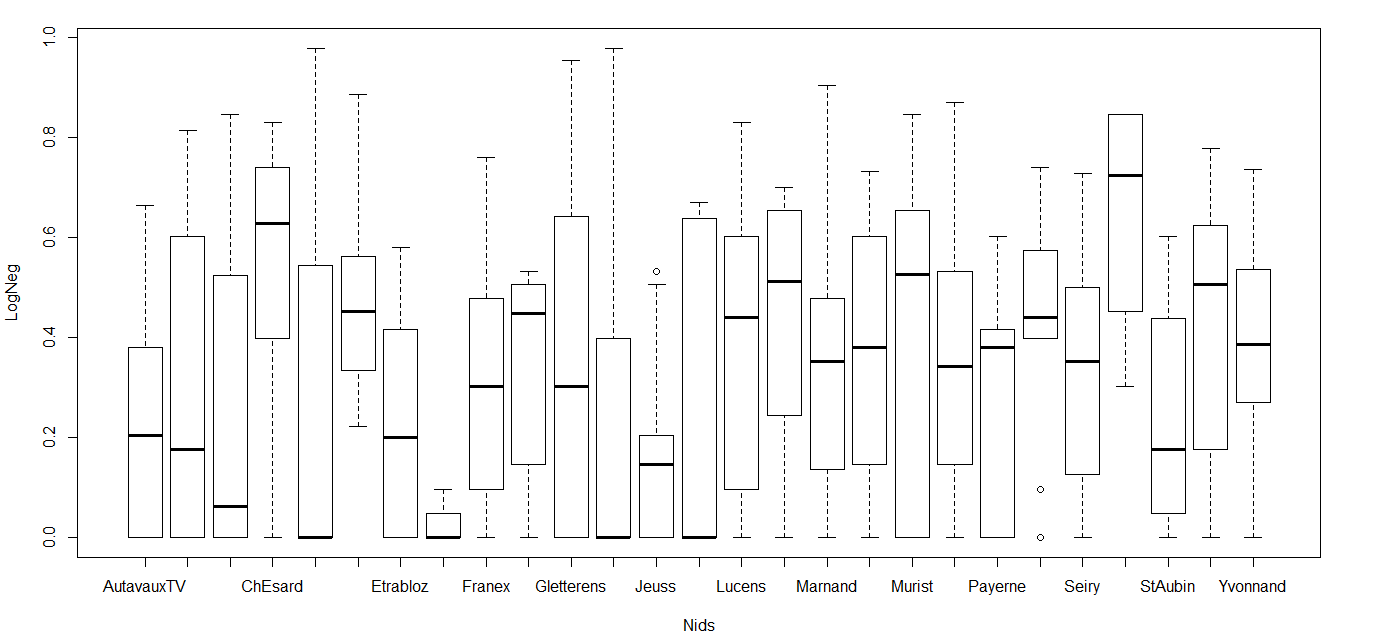
\includegraphics[scale=0.5]{Rplota}
\begin{center} Figure 1- Répartition de LogNeg en fonctions du nid\end{center}

\vspace{1em}

Dans la plupart des cas, on observe une dispersion intra-nid relativement élevée (les box-plot par nid sont assez larges), par contre la variation inter-nid est faible (exception faite pour certains nids).

\newpage

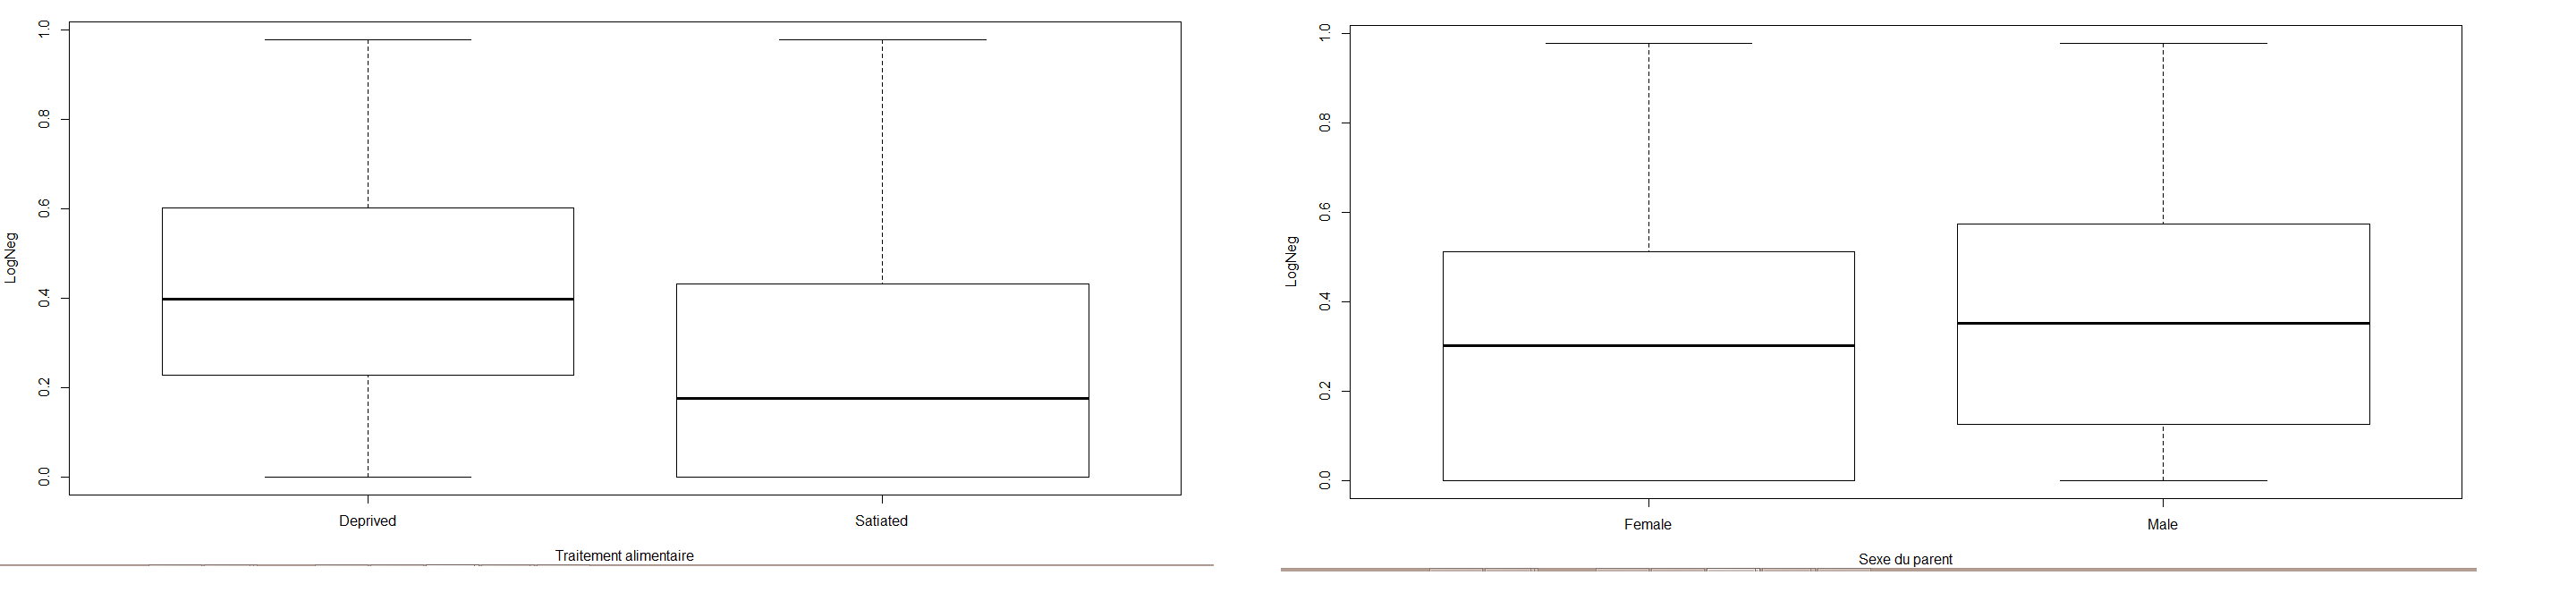
\includegraphics[scale=0.22]{Rplotb}
\begin{center} Figure 2- Répartition de LogNeg en fonction du traitement alimentaire (Deprivated\:|\:Satiated), puis en fonction du sexe des parents (Female\:|\:Male)\end{center}

\vspace{2em}

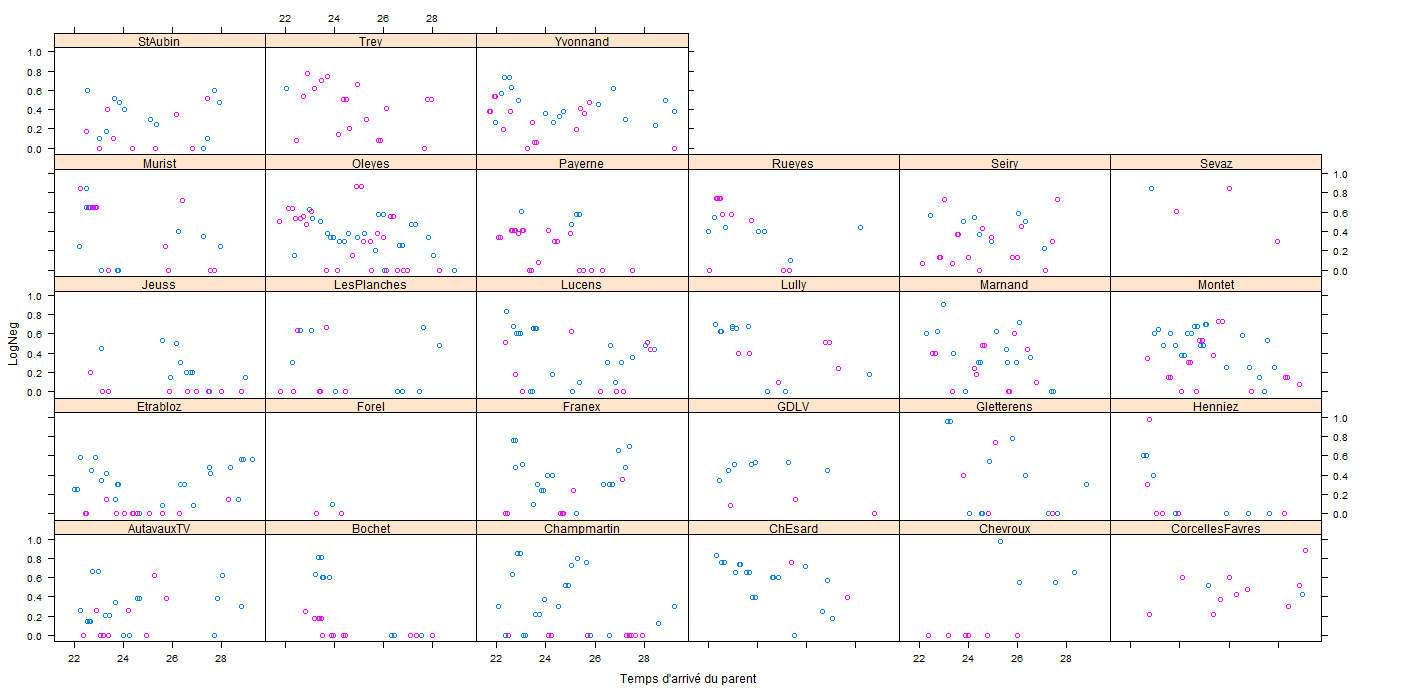
\includegraphics[scale=0.5]{Rplotc}
\begin{center} Figure 3- Répartition de LogNeg en fonction du temps d'arrivé du parent, par traitement alimentaire (Satiated en mangenta  et Deprived en bleu) et par nid \end{center}

\vspace{2em}

On constate que dans la majorité des nids le traitement alimentaire des oisillons a été varié. Cependant dans certains nids les oisillons ont recus un traitement alimentaire exclusif, c'est à dire soit ils ont été totalement privés de nourriture, soit ils ont été absolument rassasiés.

 
\newpage

\section{Illustration de la régression linéaire mixte avec la méthode ML }

\vspace{1em}

\subsection{Selection des variables} 

\vspace{1em}

\underline{\textbf{Etape 1 : Modèle complet}}

\vspace{2em}

\fcolorbox{ocre}{lightgray}{\parbox{\dimexpr \linewidth-2\fboxsep-2\fboxrule}{
\textbf{
> \: form\:=\:formula(\:LogNeg\:$\sim$\:FoodTreatment\:+\:SexParent\:+\:ArrivalTime\:+\\
FoodTreatment*SexParent\:+\:ArrivalTime*SexParent\:)\\
> \: res.ml\:=\:lme(\:form,\: random=\:$\sim$ 1\:|\:Nest,\: method="ML",\: data=Owls\:)\\
> \: summary(\:res.ml\:)
}
}}

\vspace{2em}

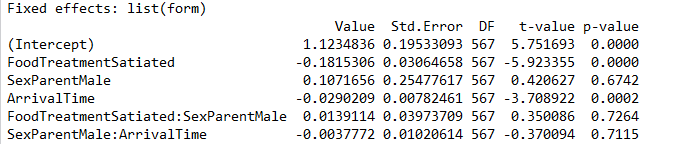
\includegraphics[scale=1]{sca}

\vspace{1em}

On remarque que les variables SexParentMale, Foodtreatment:Sex et ArrivalTime:Sex ne sont pas significatives. On va comparer le modèle complet avec d'abord le sous-modèle \textbf{a)} sans la variable Foodtreatment:Sex, puis avec le sous-modèle  \textbf{b)} sans la variable ArrivalTime:Sex. 

\vspace{2em}

\fcolorbox{ocre}{lightgray}{\parbox{\dimexpr \linewidth-2\fboxsep-2\fboxrule}{
\textbf{
>\: res.mla\:=\:update(\:res.ml,\: .$\sim$. \:-\: FoodTreatment:SexParent\:)\\
>\: res.mlb\:=\:update(\:res.ml,\: .$\sim$. \:-\:SexParent:ArrivalTime\:)\\
>\: anova(\:res.ml,res.mla\:)\\
>\: anova(\:res.ml,res.mlb\:)\\
}
}}

\vspace{2em}

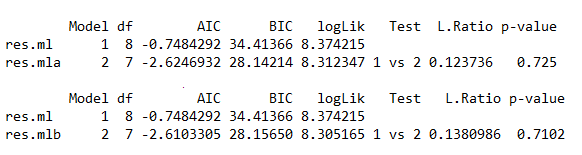
\includegraphics[scale=1]{scb}

\vspace{1em}

On accepte \textbf{(H0)} dans les deux tests car les $p$-$values$ des tests sont supérieurs à $0.05$. Et ensuite on valide l'utilisation du sous-modèle \textbf{a)} car la valeur du critère d'AIC de celui-ci est la plus faible.

\vspace{1em}

\underline{\textbf{Etape 2 : Modèle ajusté à 4 variables explicatives}}

\vspace{2em}

\fcolorbox{ocre}{lightgray}{\parbox{\dimexpr \linewidth-2\fboxsep-2\fboxrule}{
\textbf{
>\: form\:=\:formula(\:LogNeg$\sim$FoodTreatment\:+\:SexParent\:+
\:ArrivalTime\:+\\
ArrivalTime*SexParent\:)\\
>\: res.ml\:=\:lme(\:form,\: random=\:$\sim$ 1\:|\:Nest,\: method="ML",\: data=Owls\:)\\
>\: summary(\:res.ml\:)
}
}}


\vspace{2em}

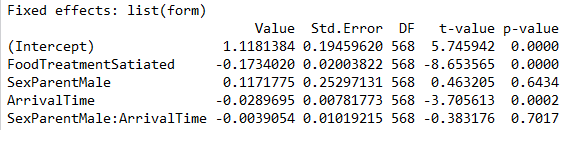
\includegraphics[scale=1]{scc}

\vspace{1em}

On remarque que les variables SexParentMale, ArrivalTime:Sexe ne sont pas significatives, on va comparer le modèle ajusté avec d'abord le sous-modèle \textbf{a)} sans la variable Sex, puis avec le sous-modèle  \textbf{b)} sans la variable ArrivalTime:Sex.

\vspace{2em}

\fcolorbox{ocre}{lightgray}{\parbox{\dimexpr \linewidth-2\fboxsep-2\fboxrule}{
\textbf{
>\: res.mla\:=\:update(\:res.ml, \:.$\sim$.\: -\: SexParent\:)\\
>\:res.mlb\:=\:update(\:res.ml, \:.$\sim$.\: -\: SexParent:ArrivalTime\:)\\
>\:anova(\:res.ml,res.mla\:)\\
>\:anova(\:res.ml,res.mlb\:)
}
}}

\vspace{2em}

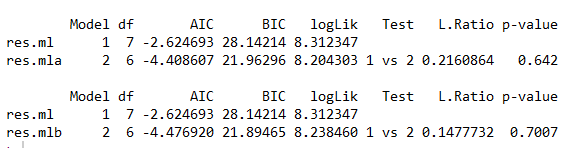
\includegraphics[scale=1]{scd}

\vspace{1em}

On accepte \textbf{(H0)} dans les deux tests car les $p$-$values$ des tests sont supérieurs à $0.05$. Et ensuite on valide l'utilisation du sous-modèle \textbf{b)} car la valeur du critère d'AIC de celui-ci est la plus faible.

\newpage

\underline{\textbf{Etape 3 : Modèle ajusté à 3 variables explicatives}}

\vspace{2em}

\fcolorbox{ocre}{lightgray}{\parbox{\dimexpr \linewidth-2\fboxsep-2\fboxrule}{
\textbf{
>\:form\:=\:formula(\:LogNeg\:$\sim$\:FoodTreatment\:+\:ArrivalTime\:+\:SexParent\:)\\
>\:res.ml\:=\:lme(\:form,\: random=\:$\sim$\:1\:|\:Nest,\: method="ML",\: data=Owls\:)\\
>\:summary(\:res.ml\:)
}
}}

\vspace{2em}

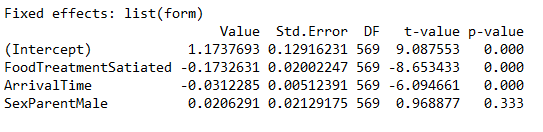
\includegraphics[scale=1]{sce}

\vspace{1em}

On remarque que la variables SexParentMale n'est pas significative, on la retire du modèle.

\vspace{1em}

\underline{\textbf{Etape 4 : Modèle selectionné}}

\vspace{2em}

\fcolorbox{ocre}{lightgray}{\parbox{\dimexpr \linewidth-2\fboxsep-2\fboxrule}{
\textbf{
>\:form\:=\:formula(\:LogNeg\:$\sim$\:FoodTreatment\:+\:ArrivalTime\:)\\
>\:res.ml\:=\:lme(\:form,\: random=\:$\sim$\:1\:|\:Nest,\: method="ML",\: data=Owls\:)\\
>\:summary(\:res.ml\:)
}
}}

\vspace{2em}

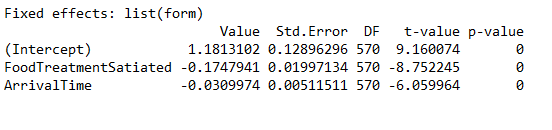
\includegraphics[scale=1]{Rplotd}

\vspace{1em}

Toutes les variables sont très significatives, le traitement alimentaire et le temps d'arrivé du parent dans le nid ont une influence sur la variable LogNeg.

\newpage

\subsection{Interprétation des résultats}

\vspace{2em}

\fcolorbox{ocre}{lightgray}{\parbox{\dimexpr \linewidth-2\fboxsep-2\fboxrule}{
\textbf{
> \:form\:=\:formula(\:LogNeg\:$\sim$\:FoodTreatment\:+\:ArrivalTime\:)\\
> \:res.ml\:=\:lme(\:form, \:random\:=\:$\sim$\:1\:|\:Nest, \:method="ML"\:,\: data=Owls\:)\\
> \:summary(\:res.ml\:)\\
}
}}

\vspace{4em}

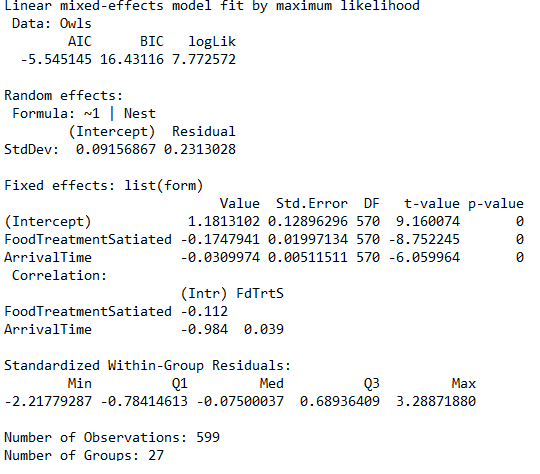
\includegraphics[scale=1]{sa}

\vspace{2em}

Avant d'aller plus loin, vérifions que nos hypothèses sont raisonnables en examinant la droite de Henry des résidus et celle pour les effets aléatoires.


\newpage

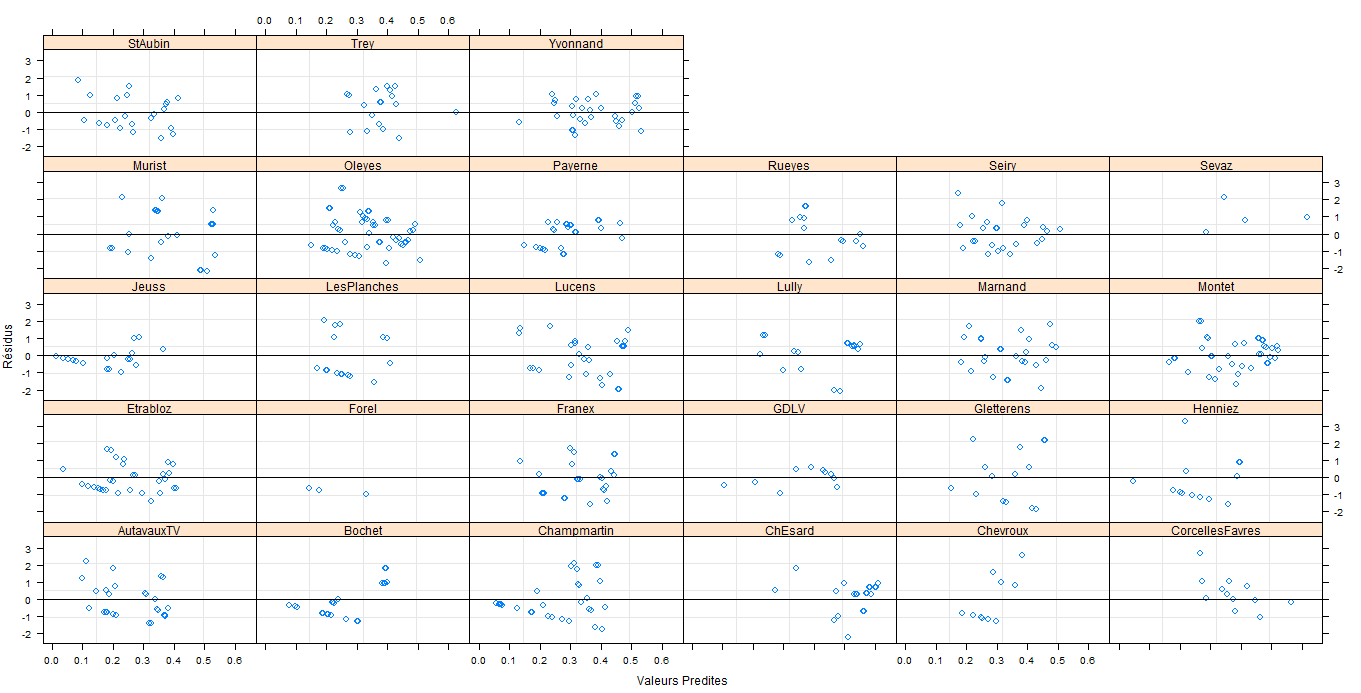
\includegraphics[scale=0.45]{Rplote}
\begin{center} Figure 4-  Les résidus en fonction des valeurs prédites par nid  \end{center}

\vspace{2em}

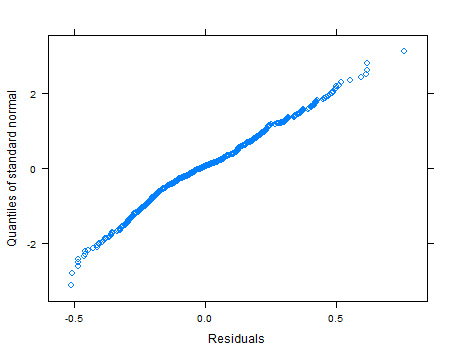
\includegraphics[scale=0.7]{Rploty}
\begin{center} Figure 5- Droite de Henry des résidus    \end{center}

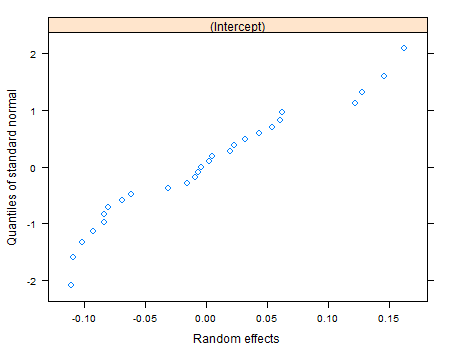
\includegraphics[scale=0.7]{Rplotw}
\begin{center} Figure 6- Droite de Henry des effets aléatoires  \end{center}

\vspace{2em}

Les résidus semblent bien centrés sur zéro et ils se situent dans une bande pour chaque nid (voir Fig. 4).
Mis à part les effets de bords inévitables, les droites de Henry (Fig. 5 et 6) montrent des points globalement alignés. Les hypothèses de normalité semblent donc raisonnables. Les hypothèses que nous avons faites semblent donc réalistes.

\newpage

\underline{\textbf{Intervalles de confiance approximatifs pour les paramètres du modèle linéaire à effets mixtes}}

\vspace{0.5em}

On utilise une approximation normale de la distribution des estimateurs du maximum de vraisemblance pour construire les intervalles de confiance approximatifs.

\vspace{2em}

\fcolorbox{ocre}{lightgray}{\parbox{\dimexpr \linewidth-2\fboxsep-2\fboxrule}{
\textbf{
>\:intervals(res.ml)
}
}}

\vspace{2em}

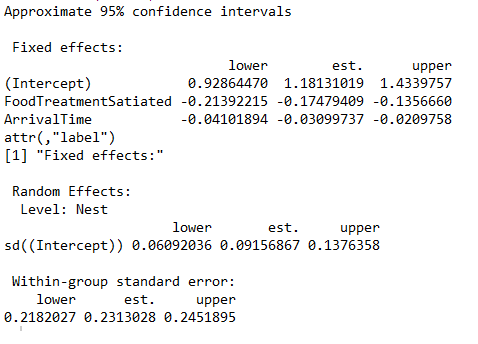
\includegraphics[scale=1]{sb}

%%%%%%%%%%%%%%%%%%%%%%%%%%%%%%%%%%%%%%%%%%%%

\newpage

\section{Illustration de la régression linéaire mixte avec la méthode REML }

\vspace{2em}

\fcolorbox{ocre}{lightgray}{\parbox{\dimexpr \linewidth-2\fboxsep-2\fboxrule}{
\textbf{
> \:form\:=\:formula(\:LogNeg\:$\sim$\:FoodTreatment\:+\:ArrivalTime\:)\\
> \:res.ml\:=\:lme(\:form, \:random\:=\:$\sim$\:1\:|\:Nest, \:method="ML"\:,\: data=Owls\:)\\
> \:summary(\:res.ml\:)\\
}
}}

\vspace{4em}

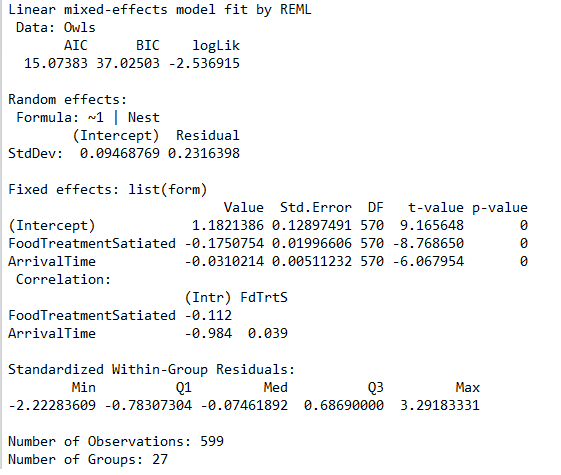
\includegraphics[scale=1]{sc}

\vspace{2em}

Les résultats obtenus sont très proches de ceux que nous avons trouvés lors de l'utilisation de la méthode ML. Une interprétation complémentaire est proposée p. 138-139 du livre "Mixed Effects Models and Extensions in Ecology with R" (réf Alain F.Zuur,...$^{\textbf{[1]}}$).



% ----------------------------------------------------------------------------------------
% 	BIBLIOGRAPHY
% ----------------------------------------------------------------------------------------

\begin{thebibliography}{9}

  \bibitem{1}
           Alain F.Zuur, Elena N.Ieno, Neil J.Walker, Anatoly A.Saveliev, Graham M.Smith,
          \emph{Mixed Effects and Extensions in Ecology with R}.
          Springer,
          129-142,
          2009.     
     
       \bibitem{2}
           Laird, N.M and Ware,J.H,
          \emph{Random effects models for longitudinal data}.
          Biometrics,
          Vol. 38, No. 4,
          963-974,
          1982.
          
          
              \bibitem{3}
           Laurent DAVEZIES,
          \emph{Modèles à effets fixes, à effets aléatoires, modèles mixtes ou multi-niveaux :
propriétés et mises en oeuvre des modélisations
de l’hétérogénéité dans le cas de données groupées}.
          60-70,
          G 2011 / 03.
 \url{http://www.crest.fr/ckfinder/userfiles/files/Pageperso/ldavezies/WorkingPaperINSEE/G2011-03.pdf}
 
 
    \bibitem{4}
           Geert Verbeke, Geert Molenberghs
          \emph{Linear Mixed Models for Longitudinal Data}.
          Springer Series in Statistics,
          QA279, V458, 2000,
          42-46,
          2009.
          
             \bibitem{5}
           Henderson C.R, Kempthorne O, Searle S.R, von Krosigk C.M,
          \emph{The estimation of
environmental and genetic trends from records subject to culling}.
          Biometrics,
          Vol. 15, No. 2.
          192-218,
          1959.
          
          
             \bibitem{6}
           Jean-Louis Foulley,
          \emph{Le modèle linéaire mixte}.
          35-40,
          2003.
          \url{http://pbil.univ-lyon1.fr/members/fpicard/franckpicard_fichiers/pdf/cours.foulley.pdf}
       
          
          
              \bibitem{7}
           V. Monbet,
          \emph{Notes de cours
Statistique inférentielle : Tests
Master Statistique et Économétrie}.
		  Univ. Rennes 1,
          Master 1,
          20-21
          2013. 
          
          
  \bibitem{8}
             Z. Griliches and M.D. Intriligator,
          \emph{Handbook of Econometrics, Volume II}.
          Elseoier Science Publishers BV,
          Chapter 13,
          773-785, 
          1984.
          
          

     



\end{thebibliography}


   




\end{document}